% TODO
%
% - Refer to Efimov
% - Discuss cohomology classes in Dyckerhoff

\documentclass[english,letter paper,12pt,leqno]{article}
\usepackage{array}
\usepackage{stmaryrd}
\usepackage{amsmath, amscd, amssymb, mathrsfs, accents, amsfonts,amsthm}
\usepackage[all]{xy}
\usepackage{dsfont}
\usepackage{tikz}
\def\nicedashedcolourscheme{\shadedraw[top color=blue!22, bottom color=blue!22, draw=gray, dashed]}
\def\nicecolourscheme{\shadedraw[top color=blue!22, bottom color=blue!22, draw=white]}
\def\nicepalecolourscheme{\shadedraw[top color=blue!12, bottom color=blue!12, draw=white]}
\def\nicenocolourscheme{\shadedraw[top color=gray!2, bottom color=gray!25, draw=white]}
\def\nicereallynocolourscheme{\shadedraw[top color=white!2, bottom color=white!25, draw=white]}
\definecolor{Myblue}{rgb}{0,0,0.6}
\usepackage[a4paper,colorlinks,citecolor=Myblue,linkcolor=Myblue,urlcolor=Myblue,pdfpagemode=None]{hyperref}

\SelectTips{cm}{}

\setlength{\evensidemargin}{0.1in}
\setlength{\oddsidemargin}{0.1in}
\setlength{\textwidth}{6.3in}
\setlength{\topmargin}{0.0in}
\setlength{\textheight}{8.5in}
\setlength{\headheight}{0in}

\newtheorem{theorem}{Theorem}[section]
\newtheorem{proposition}[theorem]{Proposition}
\newtheorem{lemma}[theorem]{Lemma}
\newtheorem{corollary}[theorem]{Corollary}
\newtheorem{setup}[theorem]{Setup}

% Labels in tabular
\newcommand{\tagarray}{\mbox{}\refstepcounter{equation}$(\theequation)$}

\newtheoremstyle{example}{\topsep}{\topsep}
	{}
	{}
	{\bfseries}
	{.}
	{2pt}
	{\thmname{#1}\thmnumber{ #2}\thmnote{ #3}}
	
	\theoremstyle{example}
	\newtheorem{definition}[theorem]{Definition}
	\newtheorem{example}[theorem]{Example}
	\newtheorem{remark}[theorem]{Remark}
	\newtheorem{strat}[theorem]{Strategy}

\numberwithin{equation}{section}

% Operators
\def\eval{\operatorname{ev}}
\def\res{\operatorname{Res}}
\def\Coker{\operatorname{Coker}}
\def\Ker{\operatorname{Ker}}
\def\im{\operatorname{Im}}
\def\can{\operatorname{can}}
\def\K{\mathbf{K}}
\def\D{\mathbf{D}}
\def\N{\mathbf{N}}
\def\LG{\mathcal{LG}}
\def\Ab{\operatorname{Ab}}
\def\stab{\operatorname{stab}}
\def\Hom{\operatorname{Hom}}
\def\modd{\operatorname{mod}}
\def\Modd{\operatorname{Mod}}
\def\be{\begin{equation}}
\def\ee{\end{equation}}
\def\nN{\mathds{N}}
\def\nZ{\mathds{Z}}
\def\nQ{\mathds{Q}}
\def\nR{\mathds{R}}
\def\nC{\mathds{C}}
\def\jac{\operatorname{Jac}_W}
\DeclareMathOperator{\Ext}{Ext}
\DeclareMathOperator{\Tr}{Tr}
\DeclareMathOperator{\End}{End}
\DeclareMathOperator{\rank}{rank}
\DeclareMathOperator{\tot}{Tot}
\DeclareMathOperator{\ch}{ch}
\DeclareMathOperator{\str}{str}
\DeclareMathOperator{\mf}{mf}
\DeclareMathOperator{\hmf}{hmf}
\DeclareMathOperator{\HMF}{HMF}
\DeclareMathOperator{\hf}{HF}
\DeclareMathOperator{\At}{At}
\DeclareMathOperator{\Cat}{Cat}
\DeclareMathOperator{\Spec}{Spec}
\DeclareMathOperator{\id}{id}
\DeclareMathOperator{\Con}{Con}

\begin{document}

% Commands
\def\Res{\res\!}
\newcommand{\ud}{\mathrm{d}}
\newcommand{\Ress}[1]{\res_{#1}\!}
\newcommand{\cat}[1]{\mathcal{#1}}
\newcommand{\lto}{\longrightarrow}
\newcommand{\xlto}[1]{\stackrel{#1}\lto}
\newcommand{\md}[1]{\mathscr{#1}}
\def\sus{\l}
\def\l{\,|\,}
\def\sgn{\textup{sgn}}
\def\samp{\zeta}
\def\Samp{Z}
\def\traff{N}

\title{$A_\infty$-categories of matrix factorisations}
\author{Daniel Murfet}

\maketitle

\begin{abstract}
We study $A_\infty$-categories associated to the DG-category of matrix factorisations.
\end{abstract}

% \tableofcontents

In this paper we study those $A_\infty$-categories which are obtained from DG-categories of matrix factorizations by the minimal model construction. This problem has been studied in various forms by several authors, including Seidel \cite{??}, Dyckerhoff \cite{??}, Efimov \cite{??} and Sheridan \cite{??}. Our point of view diverges the existing literature in that we genuinely seek to understand the full $A_\infty$-category of matrix factorisations and not just the minimal model of the endomorphism DG-algebra of a generator. Our motivation for pursuing the problem in this generality is twofold. Firstly, this is a convenient framework for studying simultaneous deformations of singularities and their matrix factorizations, as it is often inconvenient to explicitly present a given matrix factorization as a twisted complex over the generator (essentially due to the role of idempotents). Secondly, there is interesting work in this generality in the physics literature, which deserves further study.

Our approach is based on the techniques introduced in [?] and developed in [?,?]. We adjoin to the DG-category $\md{C} = \mf(R,W)$ of finite-rank matrix factorizations of a potential $W \in k[x_1,\ldots,x_n]$ over an arbitrary base ring $k$ a number of odd supercommuting variables $\theta_1,\ldots,\theta_n$ and complete along the the critical locus to obtain the DG-category
\[
\md{C}_\theta = \bigwedge F_\theta \otimes_k \md{C} \otimes_R \widehat{R}\,,
\]
where $F_\theta$ is the $\nZ_2$-graded $k$-module $\oplus_{i=1}^n k \theta_i$ which is concentrated in odd degree. The differential on the DG-category $\md{C}_\theta$ is just the one inherited from $\mathscr{C}$.

While there is no obvious strong deformation retract on $\md{C}$ which would allow one to run the minimal model construction, the DG-category $\md{C}_\theta$ can be equipped with a natural strong deformation retract which arises from differentiating in the normal directions to the critical locus (since the critical locus may not be reduced, this is admittedly a strange form of differentiation). This puts $\md{C}_\theta$ in homotopy equivalence with the tensor product
\be\label{eq:tensor_introa}
\md{C} \otimes_R \jac = \Big\{ \Hom_R(X,Y) \otimes_R \jac \big| X,Y \in \mathscr{C} \Big\}
\ee
viewed as a collection of $\nZ_2$-graded complexes of finitely-generated free $k$-modules. The usual $A_\infty$-minimal model construction equips this collection of graded modules with an $A_\infty$-structure $\{m_n\}_n$, the $m_1$ and $m_2$ of which are the differential and product that is given by interpreting \eqref{eq:tensor_introa} as a tensor product of DG-categories, with $\jac$ given the zero differential and its usual algebra structure.

Not all minimal models are created equal, since without a good grasp on the combinatorics of the homotopy which is part of the strong deformation retract, it is hopeless to try and understand the higher products which are produced. However, the strong deformation retract involved in the above construction is of a standard kind, so that the higher products may be described by a small collection of local ``Feynman rules''. 

The final step is to obtain a minimal $A_\infty$-category quasi-isomorphic to $\md{C}$ from the $A_\infty$-structure on $\md{C} \otimes_R \jac$. For this we observe that the algebra morphism 
\[
\bigwedge F_\theta \lto k \cdot 1 \lto \bigwedge F_\theta
\]
which projects onto the identity by sending all $\theta$-forms of nonzero degree to zero, gives rise to a strictly idempotent DG-functor
\[
e: \md{C}_\theta \lto \md{C}_\theta
\]
and thus by transfer to a homotopy idempotent $A_\infty$-functor
\[
\widetilde{e}: \md{C} \otimes_R \jac \lto \md{C} \otimes_R \jac\,.
\]
A minimal model for $\md{C}$ exists over $k$ (which we recall, is not a field) if and only if this idempotent splits, and so the algorithm for splitting this idempotent is an algorithm for producing the minimal model. In some sense the tuple $(\md{C} \otimes_R \jac, \{m_n\}_{n \ge 1}, \widetilde{e})$ presents the minimal model of $\md{C}$ in terms of polynomial functions of the input data - namely, the differentials in all the matrix factorizations of $W$. Calculating beyond this point involves Gaussian eliminations and thus regular functions of the input data - the output and nature of the cohomology classes varies across strata defined by the vanishing of the denominators in such functions. 

In particular, the cohomology $H^*( \md{C} \otimes_R \jac )$, the induced $A_\infty$ structure on this cohomology, and the splitting of the induced (strictly) idempotent $A_\infty$-functor $H^*(\widetilde{e})$ cannot typically be presented by universal formulas which are polynomial in the entries of the twisted differentials. 

Nonetheless these calculations may be done and $A_\infty$ minimal models of $\md{C}$ (or particularly interesting DG-subcategories of $\md{C}$) may be computed. This paper is the first in a series, and presents only the general theory with no concrete examples. In the second paper together with Patrick Elliott we will present examples, both of the minimal models of the DG-algebra $\End(k^{\stab})$ for the case of an isolated singularity and the generator, minimal models of DG-modules of the form $\Hom(k^{\stab}, X)$, and other examples involving the versal deformation of $A_n$-singularities and minimal models of DG-algebras $\End(X)$ for some interesting examples of matrix factorizations (and bifactorisations, such as the permutation defects of [?]).

\newpage

\section{Background}

\subsection{Notation}

Throughout $k$ is a commutative $\mathbb{Q}$-algebra. If $\bold{x} = (x_1,\ldots,x_n)$ is a sequence of formal variables then $k[\bold{x}]$ denotes $k[x_1,\ldots,x_n]$ and similarly for power series rings. Given $M \in \mathbb{N}^n$ we write $x^M$ for $x_1^{M_1} \cdots x_n^{M_n}$.

\subsection{Algebra}

Let $R$ be a commutative ring. Given finite-rank free $\nZ_2$-graded $R$-modules $M, N$ and $\phi \in \Hom_R(M,N)$ we say that $\phi$ is \emph{even} (resp. \emph{odd}) if $\phi(M_i) \subseteq N_i$ (resp. $\phi(M_i) \subseteq N_{i+1}$) for all $i \in \nZ_2$. This makes $\Hom_R(M,N)$ into a $\nZ_2$-graded $R$-module. Given two homogeneous operators $\psi, \phi$ the \emph{graded commutator} is
\be
[\phi, \psi] = \phi \psi - (-1)^{|\phi||\psi|} \psi \phi\,.
\ee
In this note all operators are given a $\nZ_2$-grading and the commutator always denotes the graded commutator. We often make implicit use of the graded Jacobi identity
\be\label{eq:graded_jacobi}
(-1)^{|\alpha||\gamma|}\big[ \alpha, [\beta, \gamma]\big] + (-1)^{|\alpha||\beta|}\big[ \beta, [\gamma, \alpha] \big] + (-1)^{|\gamma||\beta|} \big[ \gamma, [\alpha, \beta] \big] = 0\,.
\ee
Among the most important examples are the exterior algebras
\[
M = \bigwedge \bigoplus_{i=1}^r R \varepsilon_i
\]
where $F = \bigoplus_{i=1}^r k \varepsilon_i$ denotes a free $R$-module of rank $r$ with basis $\varepsilon_1,\ldots,\varepsilon_r$. We give $F$ a $\nZ_2$-grading by assigning $|\varepsilon_i| = 1$, that is, $F \cong R^{\oplus r}[1]$. The inherited $\nZ_2$-grading on $\bigwedge F$ is the reduction mod $2$ of the usual $\nZ$-grading on the exterior algebra, e.g. $|\varepsilon_1 \varepsilon_2| = 0$.

We define odd operators $\varepsilon_j \wedge (-), \varepsilon_j^* \,\lrcorner\, (-)$ on $\bigwedge F$ by wedge product and contraction, respectively, where contraction is defined by the formula
\begin{align*}
\varepsilon_j^* \,\lrcorner\, \Big( \varepsilon_{i_1} \cdots \varepsilon_{i_s} \Big) = \sum_{l=1}^s (-1)^{l-1} \delta_{j, i_l} \varepsilon_{i_1} \wedge \cdots \wedge \widehat{ \varepsilon_{i_l} } \wedge \cdots \wedge \varepsilon_{i_s}\,.
\end{align*}
Often we will simply write $\varepsilon_j$ for $\varepsilon_j \wedge (-)$ and $\varepsilon_j^*$ for $\varepsilon_j^* \,\lrcorner\, (-)$. Clearly with this notation, as operators on $\bigwedge F$, we have the commutator
\be\label{eq:wedge_contract_comm}
\big[ \varepsilon_i, \varepsilon_j^* \big] = \delta_{ij} \cdot 1\,.
\ee

\subsection{Quasi-regular sequences and connections}

In this section we recall the definition of quasi-regular sequences and potentials, and explain the geometric content of the connections which play a crucial role in the construction of strong deformation retracts in the body of the paper. For more on the theory of quasi-regular sequences see \cite{matsumura}, \cite[Chapitre $0$ \S 15.1]{EGA4} and \cite[Section\,10.68]{stacks_project}.

\begin{definition} A sequence $t_1,\ldots,t_n$ in a commutative ring $R$ is \emph{quasi-regular} if, writing $I = (t_1,\ldots,t_n)$, the morphism of $R/I$-algebras
\begin{gather*}
\phi: R/I[z_1,\ldots,z_n] \lto \operatorname{gr}_I R = \bigoplus_{i \ge 0} I^i / I^{i+1}\\
\phi(z_i) = \overline{t_i} \in I/I^2
\end{gather*}
is an isomorphism. In particular, this means that $I/I^2 \cong \bigoplus_{i=1}^n R/I \cdot \overline{t_i}$.
\end{definition}

We briefly recall the motivation for this definition from algebraic geometry.

\begin{remark} Let $Y$ be a noetherian scheme and let $i: X \lto Y$ be a closed subscheme with ideal sheaf $\mathscr{I}$. As in differential geometry the first-order deformations of $X$ in $Y$ are controlled \cite[Theorem VI-29]{eisenbudharris} by the normal sheaf
\[
\mathscr{N}_{X/Y} = \Hom_{\cat{O}_X}(\mathscr{I}/\mathscr{I}^2, \cat{O}_X).
\]
However, to correctly describe the space of normal directions to $X$ in $Y$ beyond first-order requires more than just the normal sheaf. The correct approach is to start with the blowup $\pi$ of $Y$ along $X$ which is described by a universal property, and then look at the closed subscheme of that blowup induced by $X$ as in the diagram:
\[
\xymatrix@C+2pc{
\operatorname{Proj}_X( \oplus_{i \ge 0} \mathscr{I}^i/\mathscr{I}^{i+1} ) \ar[r]^-j\ar[d] & \operatorname{Proj}_Y( \oplus_{i \ge 0} \mathscr{I} ) \ar[d]^-{\pi}\\
X \ar[r]_-{i} & Y\,.
}
\]
The closed subscheme $j$ of the blowup (called the strict transform of $X$) is given by the relative Proj of the sheaf of graded algebras $\oplus_{i \ge 0} \mathscr{I}^i/\mathscr{I}^{i+1}$ on $X$, and its points give the correct notion of a point on $X$ together with a normal direction in $Y$. For this reason the scheme $C_X(Y) = \Spec_X( \oplus_{i \ge 0} \mathscr{I}^i / \mathscr{I}^{i+1} )$, whose projectivisation is the strict transform of $X$ in the blowup, is often called the \emph{normal cone} of $X$ in $Y$ \cite{??,??}.
\end{remark}

Thus, to say that a sequence $t_1,\ldots,t_n$ is quasi-regular is to say that the projectivised normal cone of $X = \Spec(R/I)$ in $Y = \Spec(R)$ is the space of lines in the normal bundle, since the definition of quasi-regularity gives 
\begin{align*}
\Spec_{Y}( \operatorname{Sym}( \mathscr{N}^*_{X/Y} ) ) &\cong \Spec( \operatorname{Sym}_{R/I}( I/I^2 ) )\\
&= \Spec( R/I[z_1,\ldots,z_n] )\\
&\cong \Spec( \operatorname{gr}_ I R)\\
&= C_X(Y)\,.
\end{align*}
Suppose we have a smooth manifold $Y$, a submanifold $X \subseteq Y$ and a smooth function $f$ on a neighborhood of $X$. We can define the derivative of $f$ in the directions normal to $X$, by putting a suitable connection on the restriction of the sheaf of smooth functions $\cat{O}_Y^\infty$ to a suitable open neighborhood of $X$. This connection can be produced by taking a tubular neighborhood, which allows us to identify a neighborhood of the zero section $X \lto N_{X/Y}$ of the normal bundle with an open neighborhood of $X$ in $Y$. 

There is no direct analogue of this identification of neighborhoods for a closed immersion $i: X \lto Y$ of schemes, even if we are in the good situation where $I = (t_1,\ldots,t_n)$ is generated by a quasi-regular sequence. To ask for such an identification, even at the level of infinitesimal neighborhoods of $X$ in the normal cone $C_X(Y)$ and $Y$ respectively, would be to task in the affine case above for an isomorphism of topological rings
\[
R/I\llbracket z_1,\ldots,z_n \rrbracket \lto \widehat{R}
\]
where $\widehat{R}$ is the $I$-adic completion. It easy to produce examples where this fails:

\begin{example} Let $k$ be a field, $R = k[x]$ and $I = (x^d)$ for $d > 1$. Since the $I$-adic topology is the same as the $(x)$-adic topology, 
\[
R/I\llbracket z \rrbracket = k[x]/(x^d) \llbracket z \rrbracket \neq k\llbracket x \rrbracket = \widehat{R}\,,
\]
since one ring is reduced while the other is not.
\end{example}

The good news is that if we only want to define a connection on the ring of functions which differentiates in the directions normal to $X$, we do not need to identify infinitesimal neighborhoods of $X$ in $C_X(Y)$ and $Y$, as the weaker statement in the following proposition will do.

\begin{setup} For the rest of this section let $R$ be a $k$-algebra, and let $t_1,\ldots,t_n$ be a quasi-regular sequence in $R$ such that, writing $I = (t_1,\ldots,t_n)$ the quotient $R/I$ is a finitely generated projective $k$-module.
\end{setup}

\begin{proposition}[Lipman]\label{prop_algtube} Any $k$-linear section $\sigma$ of the quotient $\pi: R \lto R/I$ induces an isomorphism of $k\llbracket z_1,\ldots,z_n \rrbracket$-modules
\[
\sigma^*: R/I \otimes_k k\llbracket z_1,\ldots,z_n \rrbracket \lto \widehat{R}
\]
where $\widehat{R}$ denotes the $I$-adic completion.
\end{proposition}
\begin{proof}
See \cite{??}. Given a section $\sigma$ the map $\sigma^*(s \otimes z^M) = \sigma(s) t^M$ is induced by extension of scalars, making $\widehat{R}$ a $k\llbracket \bold{z} \rrbracket$-module by making $z_i$ act as multiplication by $t_i$. The main point is that every $r \in \widehat{R}$ has a \emph{unique} representation as a power series
\be\label{eq:uniq_decompr}
r = \sum_{M \in \mathbb{N}^n} \sigma(r_M) t^M
\ee
for elements $r_M \in R/I$, and the inverse to $\sigma^*$ sends $r$ to $\sum_M r_M z^M$.
\end{proof}

Recall from \cite{??} the notion of a $k$-linear connection on a module over a $k$-algebra. As alluded to above, we can use the isomorphism of Lemma \ref{??} to produce connections.

\begin{corollary} Associated to any $k$-linear section $\sigma$ is a $k$-linear connection
\be
\nabla_\sigma: \widehat{R} \lto \widehat{R} \otimes_{k[\bold{z}]} \Omega^1_{k[\bold{z}]/k}
\ee
on $\widehat{R}$ as a $k[\bold{z}]$-module.
\end{corollary}
\begin{proof}
The usual partial derivatives give a $k$-linear connection on $k\llbracket \bold{z} \rrbracket$ as a $k[\bold{z}]$-module which extends, by Propositon \ref{prop_algtube}, to a connection on $\widehat{R}$. In terms of the power series representation \eqref{eq:uniq_decompr} it is given by
\be
\nabla_\sigma(r) = \sum_{j=1}^n \sum_{M \in \mathbb{N}^n} M_j \sigma(r_M) t^{M - e_j} \otimes dz_j\,.
\ee
\end{proof}
The functions $f \in \widehat{R}$ which are ``constant'' in the normal directions according to this connection, that is, which satisfy $\nabla_\sigma(f) = 0$, are precisely those in the image of the section $\sigma$. There is no ``intrinsic'' derivative of $f$ which is independent of choices, but the various algebraic constructions we perform using the connection $\nabla_\sigma$ will be independent of the choice of section $\sigma$ up to homotopy, nonetheless.

\begin{remark} With a section $\sigma$ fixed, we will typically abuse notation and write $\nabla$ for the associated connection. We also introduce $k$-linear operators $\frac{\partial}{\partial z_i}: \widehat{R} \lto \widehat{R}$ by the identity
\[
\nabla = \sum_{j=1}^n \frac{\partial}{\partial z_i} dz_j \,.
\]
Typically we write $\partial_{z_i}$ for these operators. In practice we think of this operator as $\frac{\partial}{\partial t_i}$, and this notation, while misleading, is helpful.
\end{remark}

\begin{example} Let $k$ be a field, $R = k[x]$ and $I = (x^d)$, with $t = x^d$. Choose the $k$-linear section
\[
\sigma: R/I \lto R\,, \qquad \sigma(x^i) = x^i \quad 0 \le i \le d - 1\,,
\]
and let $\nabla_\sigma$ be the associated connection. Then
\[
\frac{\partial}{\partial z}( x^2 + x^{d+1} ) = \frac{\partial}{\partial z}( x^2 \cdot 1 + x \cdot x^d ) = x\,.
\]
\end{example}

From the point of view of homological algebra, the Koszul complex 
\[
K(R, \bold{t}) = \Big( \bigwedge( k \theta_1 \oplus \cdots \oplus k \theta_n ) \otimes_k R, \,\,\sum_i t_i \theta_i^* \Big)
\]
is a a projective resolution of the $R$-algebra $R/I$ in the world of DG-$R$-algebras. Once we complete in the $I$-adic topology the relationship between these two DG-algebras becomes even stronger: there is a $k$-linear \emph{homotopy equivalence}
\[
K(\widehat{R}, \bold{t}) \lto \widehat{R}/I\widehat{R} = R/I\,.
\]
A connection of the form $\nabla_\sigma$ is the only natural way of writing down the data which defines this homotopy equivalence. This homotopy equivalence gives us a much more flexible model of $R/I$, which may be used for example in the setting of the perturbation lemma.

\begin{definition} A \emph{strong deformation retract} over a commutative ring $S$ is a pair of morphisms of $\mathbb{Z}_2$-graded complexes of $S$-modules $\pi, \sigma$ as in the diagram
\begin{equation}\label{eq:defn_sdr}
\xymatrix@C+3pc{
(M,d) \ar@<-1ex>[r]_\sigma & (A,d)\,, \ar@<-1ex>[l]_\pi
}\quad \phi
\end{equation}
together with an odd $S$-linear operator $\phi: A \lto A$ satisfying
\begin{itemize}
\item[(i)] $\pi \sigma = 1_M$,
\item[(ii)] $\sigma \pi = 1_A - [d, \phi]$,
\item[(iii)] $\phi^2 = 0$,
\item[(iv)] $\phi \sigma = 0$,
\item[(v)] $\pi \phi = 0$.
\end{itemize}
\end{definition}

We adopt the following notation going forwards:
\be
F_\theta = k\theta_1 \oplus \cdots \oplus k \theta_n\,,
\ee
where we make $F_\theta$ a $\mathbb{Z}_2$-graded $k$-module by taking $|\theta_i| = 1$.

\begin{proposition} There is a strong deformation retract
\begin{equation}\label{eq:defn_sdr}
\xymatrix@C+3pc{
(R/I,0) \ar@<-1ex>[r]_-\sigma & \Big( \bigwedge F_\theta \otimes_k \widehat{R}, \,\,d_K = \sum_i t_i \theta_i^*\, \Big)\,, \ar@<-1ex>[l]_-\pi
}\quad H_\sigma
\end{equation}
where
\begin{itemize}
\item $\sigma$ is the section $R/I \lto \widehat{R}$ followed by the inclusion,
\item $\pi$ is the quotient map 
\item $H_\sigma = [\nabla, d_K]^{-1} d_K$.
\end{itemize}
\end{proposition}

\subsection{DG-categories and $A_\infty$-categories}

In this section we review standard material on DG-categories and $A_\infty$-categories, including the statement of the minimal model theorem. Our primary reference is \cite{lazaroiu}.

\begin{definition} If $\mathscr{C}, \mathscr{D}$ are DG-categories then $\mathscr{C} \otimes_k \cat{D}$ is a DG-category with
\begin{gather*}
\operatorname{ob}( \mathscr{C} \otimes_k \mathscr{D} ) = \operatorname{ob}(\mathscr{C}) \times \operatorname{ob}(\mathscr{D})\,,\\
\big( \mathscr{C} \otimes_k \mathscr{D} \big)( (C_1, D_1), (C_2, D_2) ) = \mathscr{C}(C_1, C_2) \otimes_k \mathscr{D}(D_1, D_2)
\end{gather*}
with the obvious composition. In particular if $\Lambda$ is a $\mathbb{Z}_2$-graded $k$-algebra (not necessarily commutative) then $\mathscr{C} \otimes_k R$ is a DG-category with the same objects as $\mathscr{C}$ and
\[
\big( \mathscr{C} \otimes_k R \big)( C_1, C_2 ) = \mathscr{C}(C_1, C_2) \otimes_k \Lambda\,.
\]
\end{definition}

\begin{definition} An \emph{$A_\infty$-category} $\mathscr{A}$ consists of the following data:
\begin{itemize}
\item a class $\operatorname{ob}(\mathscr{A})$ of objects,
\item for every pair of objects $a,b \in \operatorname{ob}(\mathscr{A})$ a $\mathbb{Z}_2$-graded $k$-module $\mathscr{A}(a,b)$, and
\item for any sequence $a_0,\ldots,a_n$ of objects with $n \ge 0$ a $k$-linear map
\[
\mu_{a_n,\ldots,a_0}: \mathscr{A}(a_{n-1}, a_n) \otimes_k \cdots \otimes_k \mathscr{A}(a_0, a_1) \lto \mathscr{A}(a_0,a_n)
\]
of degree $2 - n$. If it will not cause confusion we write $\mu_n$ for $\mu_{a_n,\ldots,a_0}$.
\end{itemize}
This data is subject to the following \emph{$A_\infty$-constraints}:
\begin{align*}
\sum_{\substack{i \ge 0, j \ge 1 \\ 1 \le i + j \le n }} (-1)^{ij + i + j + n} \mu_{n-j+1}\Big( x_n \otimes \cdots \otimes x_{i+j+1} \otimes \mu_j\big( x_{i+j} \otimes \cdots \\
\cdots \otimes x_{i+1} \big) \otimes x_i \otimes \cdots \otimes x_1 \Big) = 0
\end{align*}
which has to hold for all $n \ge 1$ and composable homogeneous morphisms $x_1,\ldots,x_n$.
\end{definition}

There is an equivalent definition which is often easier to work with. Instead of the linear maps $\mu_{a_n,\ldots,a_0}$ of degree $2-n$ we take the data of degree $1$ linear maps
\be
r_{a_0,\ldots,a_n}: \mathscr{A}(a_0,a_1)[1] \otimes_k \cdots \otimes_k \mathscr{A}(a_{n-1},a_n)[1] \lto \mathscr{A}(a_0,a_n)[1]
\ee
which are subject to the \emph{forward suspended $A_\infty$-constraints}, written this time in terms of an equality of linear maps:
\be
\sum_{\substack{i \ge 0, j \ge 1 \\ 1 \le i + j \le n }} r_{n-j+1}\Big( \operatorname{id}^{\otimes i} \otimes r_j \otimes \operatorname{id}^{\otimes n - i - j} \Big) = 0
\ee

\begin{itemize}
\item Definition
\item Suspended forward
\item Strict units
\item Trees and denotations
\item Minimal model theorem
\item Variant with units
\end{itemize}

\subsection{Matrix factorisations}

We recall from \cite{lgdual} the definition of a potential:

\begin{definition}\label{defn:potential} A polynomial $W \in k[x_1,\ldots,x_n]$ is a \textsl{potential} if (we write $t_i = \partial_{x_i} W$)
\begin{itemize}
\item[(i)] $t_1,\ldots,t_n$ is a quasi-regular sequence;
\item[(ii)] $k[x_1,\ldots,x_n]/(t_1,\ldots,t_n)$ is a finitely generated free $k$-module;
\item[(iii)] the Koszul complex of $t_1,\ldots,t_n$ is exact except in degree zero.
\end{itemize}
\end{definition}

A typical example is a polynomial $W \in \mathbb{C}[x_1,\ldots,x_n]$ with isolated critical points \cite[Example ??]{lgdual}. As shown in \cite{lgdual}, these hypotheses on a potential are sufficient to produce all the properties relevant to two-dimensional topological field theory (e.g. nondegenerate pairings, adjoints, etc.). We will see in Remark \ref{??} below why the hypothesis (iii) is necessary for our methods. In any case, if $k$ is noetherian then (iii) follows from (i).
\\

Let $W \in R = k[x_1,\ldots,x_n]$ be a potential. 

\begin{definition} The DG-category $\mathscr{C} = \mf(R,W)$ has as objects \emph{matrix factorisations} of $W$ over $R$, that is, the pairs $(X, d_X)$ consisting of a $\mathbb{Z}_2$-graded finite free $R$-module $X$ and an odd $R$-linear operator $d_X: X \lto X$ satisfying $d_X^2 = W \cdot 1_X$. We define
\begin{gather*}
\mathscr{C}(X,Y) = \big( \Hom_R(X,Y) \,, d_{\mathscr{C}(X,Y)} \big)\,,\\
d_{\mathscr{C}(X,Y)}(\alpha)  = d_Y \circ \alpha - (-1)^{|\alpha|} \alpha \circ d_X\,.
\end{gather*}
The composition is the usual composition of linear maps.
\end{definition}

\begin{lemma} Let $W \in R$ be a potential. The DG-functor
\[
F: \mf(R,W) \lto \mf(R, W) \otimes_R \widehat{R}
\]
\end{lemma}
is a $k$-linear homotopy equivalence.
\begin{proof}
This uses hypothesis (iii) in the definition of a potential.
\end{proof}

\section{The strong deformation retract on $\mathscr{C}_\theta$}

From now on $k$ is a $\mathbb{Q}$-algebra and $W \in R = k[x_1,\ldots,x_n]$ is a potential. We fix a full sub-DG-category $\mathscr{C}$ of $\mf(R,W)$ and a quasi-regular sequence $t_1,\ldots,t_n$ in $R$ such that $t_i$ acts null-homotopically on $\mathscr{C}(X,Y)$ for every $X,Y \in \operatorname{ob}(\mathscr{C})$. We set $I = (t_1,\ldots,t_n)$ and we have chosen a $k$-linear section $\sigma$ of the quotient $R \lto R/I$.

The overall approach of the paper is to complete the DG-category $\mathscr{C} = \mf(R,W)$ along the critical locus, and then use connections of the form $\nabla_\sigma$ to rewrite the data in terms of a DG-category over $k$ made up of finitely generated modules over the Jacobi ring $\jac$.

Conceptually, identifying the completion $\widehat{R}$ with an infinitesimal neighborhood $\widehat{Y}_X$ of $X = \Spec(R/I)$ in $Y = \Spec(R)$ and thinking in terms of the tubular neighborhood, we use the nonexistent formal isomorphism between $\widehat{Y}_X$ and the total space of the normal bundle $\mathscr{N}_{X/Y}$ to turn $\mathscr{C}$ (viewed as some collection of bundles with structure maps over $\widehat{Y}_X$) into a collection of bundles with structure maps over $N_{X/Y}$ ($t_i$ vanishing up to homopty vs on the nose).

Let $\lambda_i$ denote an odd $R$-linear operator on $\mathscr{C}(X,Y)$ with the property that
\[
[ d_{\mathscr{C}(X,Y)}, \lambda_i ] = t_i \cdot 1_{\mathscr{C}(X,Y)}\,.
\]
Then we define
\[
\delta = \sum_{i=1}^n \lambda_i \theta_i^*\,.
\]
\begin{equation}
\xymatrix@C+3pc@R+3pc{
\Big( \bigwedge F_\theta \otimes_k \mathscr{C}(X,Y) \otimes_R \widehat{R}, \,\, d_{\mathscr{C}(X,Y)}\, \Big) \ar@<-2ex>[d]_-{\exp(-\delta)}\\
\Big( \bigwedge F_\theta \otimes_k \mathscr{C}(X,Y) \otimes_R \widehat{R}, \,\, d_{\mathscr{C}(X,Y)} + d_K\, \Big) \ar@<-2ex>[u]_-{\exp(\delta)} \ar@<-2ex>[d]_-{\pi} \\
\Big( \mathscr{C}(X,Y) \otimes_R \jac, \,\, d_{\mathscr{C}(X,Y)} \otimes 1 \Big) \ar@<-2ex>[u]_-{\sigma_\infty}
}
\end{equation}


\newpage

\begin{itemize}
\item Present perturbation
\item State theorem about existence of strong deformation retract, with a description of $H, \sigma_\infty$ etc.
\item Give $\mathscr{H}, \mathscr{K}$ with relevant operators
\item Give the overall picture diagram from our lectures
\item Recalculate tree based on A, B, C interactions
\item Present Feynman rules
\item Switch to $k^stab$ and do calculation
\end{itemize}

\newpage

Let us summarise the above, in the special case where $k$ is a field:
\[
\xymatrix@C+3pc@R+2pc{
\End_R(k^{\stab}) \ar[d] \ar[rr] & & \big( H^*\End_R(k^{\stab}), \{ m_k \}_{k \ge 2} \big) \ar[d]\\
\mathscr{C} \ar[d] \ar@{.>}[rr] & & \big( H^*\mathscr{C}, \{ m_k \}_{k \ge 2} \big) \ar[dd]\\
\mathscr{C} \otimes_R \widehat{R} \ar[d]\\
\mathscr{C}_\theta \ar[r] & \big( \mathscr{C} \otimes_R \jac, \{ m_k \}_{k \ge 1} \big) & \big( H^*( \mathscr{C} \otimes_R \jac ), \{ m_k \}_{k \ge 2} \big) \ar[l]
}
\]
In the left hand vertical column are DG-algebras and DG-categories, with all vertical arrows inclusions of DG-categories. The rows represent minimal models

\newpage

\subsection{The special case of the generator}

Suppose that $k$ is a field and that the potential $W$ belongs to $\mf{m}^3$ where $\mf{m} = (x_1,\ldots,x_n)$, choose a presentation $W = \sum_i x_i W^i$ with $W^i \in \mf{m}^2$ and consider the following pair
\begin{equation}\label{eq:kstab}
k^{\operatorname{stab}} = \Big( k[x] \otimes_k \bigwedge\big( \oplus_{i=1}^n k\psi_i \,\big), \;d_{k^{\stab}} = \sum_{i=1}^n x_i \psi_i^* + \sum_{i=1}^n W^i \psi_i \Big)
\end{equation}
where $\psi_i^*, \psi_i$ denote respectively the operators of contraction $\psi_i^* \lrcorner (-)$ and wedge product $\psi_i = \psi_i \wedge (-)$ on the exterior algebra. Clearly $(d_{k^{\stab}})^2 = W$ so that $k^{\stab}$ is a matrix factorisation of $W$. When $k$ is a field and $W$ has an isolated critical point at the origin, $k^{\stab}$ is the representative in the homotopy category of matrix factorisations of the structure sheaf of the singular point at the origin, and was first studied by Dyckerhoff \cite{d0904.4713}. If the origin is the only singular point of the zero locus of $W$, or we work with power series instead of the polynomial ring, $k^{\stab}$ is a split generator of the homotopy category of matrix factorisations \cite[Theorem ?]{?}.

The purpose of this paper is to show how to calculate the $A_\infty$-minimal model $\mathscr{B}$ of the $\nZ_2$-graded differential graded endomorphism algebra
\be\label{eq:defnaw}
\mathscr{A} = \Big( \End_{k[x]}(k^{\operatorname{stab}}), \; \partial = [d_{k^{\stab}},-] \; \Big)\,.
\ee 
The differential here is (throughout all commutators are graded commutators)
\begin{align*}
\partial = [d_{k^{\stab}},-] &= \Big[\sum_i x_i \psi_i^* + \sum_i W^i \psi_i, -\Big]\\
&= \sum_i x_i [\psi_i^*,-] + \sum_i W^i [\psi_i,-]\,.
\end{align*}
The minimal model is a finite-dimensional $\nZ_2$-graded vector space $\mathscr{B}$ with a family 
\[
\left\{ \rho_q: \big(\mathscr{B}[1]\big)^{\otimes q} \lto \mathscr{B}[1] \right\}_{q \ge 2}
\]
of odd $k$-linear maps satisfying the forward suspended $A_\infty$-constraints \cite{lazaroiu}, and having the property that there is an $A_\infty$-quasi-isomorphism $\mathscr{B} \lto \mathscr{A}$.

\section{Background}

\section{Feynman diagrams}
% from p.17 (ainfmf9)

The $A_\infty$-products on $\mathscr{B}$ are defined in terms of Feynman diagrams (see Definition \ref{defn:bainf}). In this section we explain how to enumerate all the relevant diagrams and how to compute their value; in the next section we prove that the maps they give rise to do indeed compute the minimal model of $\mathscr{A}$. As references for Feynman diagrams in physics we recommend \cite[Ch. 6]{weinberg}, \cite[\S 4.4]{ps}, while more mathematical treatments can be found in the lectures of Kazhdan and Witten in \cite{qftstring}.

Throughout $\otimes = \otimes_k$. The integer $n$ is the number of variables in the ambient ring $R = k[x_1,\ldots,x_n]$. We assume in this section that $W \in \mf{m}^3$. This is not a real restriction, as we will prove in Section \ref{??} that if $W \in \mf{m}^2$ is written in the form
\be
W = W'(x_1,\ldots,x_r) + \sum_{i={r+1}}^n \lambda_i x_i^2\,, \quad \text{ with } \quad W' \in \mf{m}^3
\ee
and if $\mathscr{B}'$ denotes the minimal model of $W'$ as constructed below, then as $A_\infty$-algebras
\be
\mathscr{B} \cong \mathscr{B}' \otimes_k C( Q )
\ee
where $C(Q)$ is the Clifford algebra of the quadratic form $Q = \sum_{i=r+1}^n \lambda_i x_i^2$, with no higher products (i.e. viewed simply as a $\nZ_2$-graded algebra). We may therefore restrict without loss of generality to $W \in \mf{m}^3$ in what follows.

\begin{definition}\label{defn:handop} Consider the $\nZ_2$-graded $k$-algebra defined by the tensor product
\be
\mathscr{H} = R \otimes_k \bigwedge\big( \oplus_{i=1}^n k \theta_i \,\big) \otimes_k \End_k\Big( \bigwedge\big( \oplus_{i=1}^n k \psi_i \, \big) \Big)
\ee
with degrees $|x_i| = 0$ and $|\theta_i| = |\psi_i| = 1$. On this space we have homogeneous operators
\be
x_i\,, \partial_i = \partial_{x_i}\,, \theta_i\,, \theta_i^*\,, \big[\psi_i\,,-\big]\,.
\ee
Here $\psi_i$ denotes the operator $\psi_i \wedge (-)$ on $\bigwedge\big( \oplus_{i=1}^n k \psi_i \, \big)$ and $[ \psi_i, - ]$ the graded commutator with this operator, defined on a homogeneous operator $\beta$ by
\[
\big[ \psi_i, \beta \big] = \psi_i \circ \beta - (-1)^{|\beta|} \beta \circ \psi_i\,.
\]
We define the $\nZ_2$-graded $k$-module
\be\label{defn:B}
\mathscr{B} = \bigwedge\big( \oplus_{i=1}^n k \psi_i^* \,\big)
\ee
with $|\psi_i^*| = 1$ which we view as a graded submodule
\[
\mathscr{B} \subset \End_k\Big( \bigwedge\big( \oplus_{i=1}^n k \psi_i \, \big) \Big)
\]
by identifying $\psi_i^* \in \mathscr{B}$ with the operation of contraction $\psi_i^*\, \lrcorner\, (-)$ on the exterior algebra. In this way we may also identify $\mathscr{B}$ with a submodule of $\mathscr{H}$, and we write $\sigma: \mathscr{B} \lto \mathscr{H}$ for the inclusion. Note that the operator $[\psi_j, -]$ on $\mathscr{H}$ defined above acts on the submodule $\mathscr{B}$ as contraction with $\psi_j = (\psi_j^*)^*$, that is,
\be\label{eq:comm_is_ann}
\Big[ \psi_j, \sigma\big(\psi_{i_1}^* \wedge \cdots \wedge \psi_{i_r}^*\big) \Big] = \sum_{l=1}^r (-1)^{l-1} \delta_{j, i_l} \sigma\big(\psi_{i_1}^* \wedge \cdots \wedge \widehat{ \psi_{i_l}^* } \wedge \cdots \wedge \psi_{i_r}^*\big)\,.
\ee
We write $p: \mathscr{H} \lto \mathscr{H}$ for the $k$-algebra endomorphism of $\mathscr{H}$ sending $x_i, \theta_i$ to zero for $1 \le i \le n$ and which is the identity on $\End_k( \wedge( \oplus_i k\psi_i ) )$.
\end{definition}

We view $\mathscr{H}$ as the tensor product of the bosonic Fock space $R$ with creation and annihilation operators $x_i, \partial_i$, fermionic Fock space $\wedge( \oplus_{i=1}^n k \theta_i )$ with creation and annihilation operators $\theta_i, \theta_i^*$ and the third factor, of which the calculations of the $A_\infty$-structure only involve the submodule $\mathscr{B} = \wedge( \oplus_{i=1}^n k \psi_i^* )$ which is another fermionic Fock space. The inputs to the Feynman diagrams are tensor products of states in $\mathscr{B}$, that is, wedge products of $\psi_i^*$'s, on which the $[\psi_i, -]$ act as annihilation operators.

The linear maps in \eqref{eq:int_input}, \eqref{eq:int_intedge}, \eqref{eq:int_intvert} below which determine the $A_\infty$ products $\rho_q$ on $\mathscr{B}$ will be defined in terms of these creation and annihilation operators on $\mathscr{H}$, and may be interpreted as particle interactions in the usual way. The interactions that appear are the following ones, depicted on the left as Feynman diagrams and on the right as operators. We call these respectively \emph{A-, B- and C-type interactions}:

\begin{center}
\begin{tabular}{ >{\centering}m{1cm} >{\centering}m{4cm} >{\centering}m{8cm} >{\centering}m{1cm}}
\textbf{A}
&
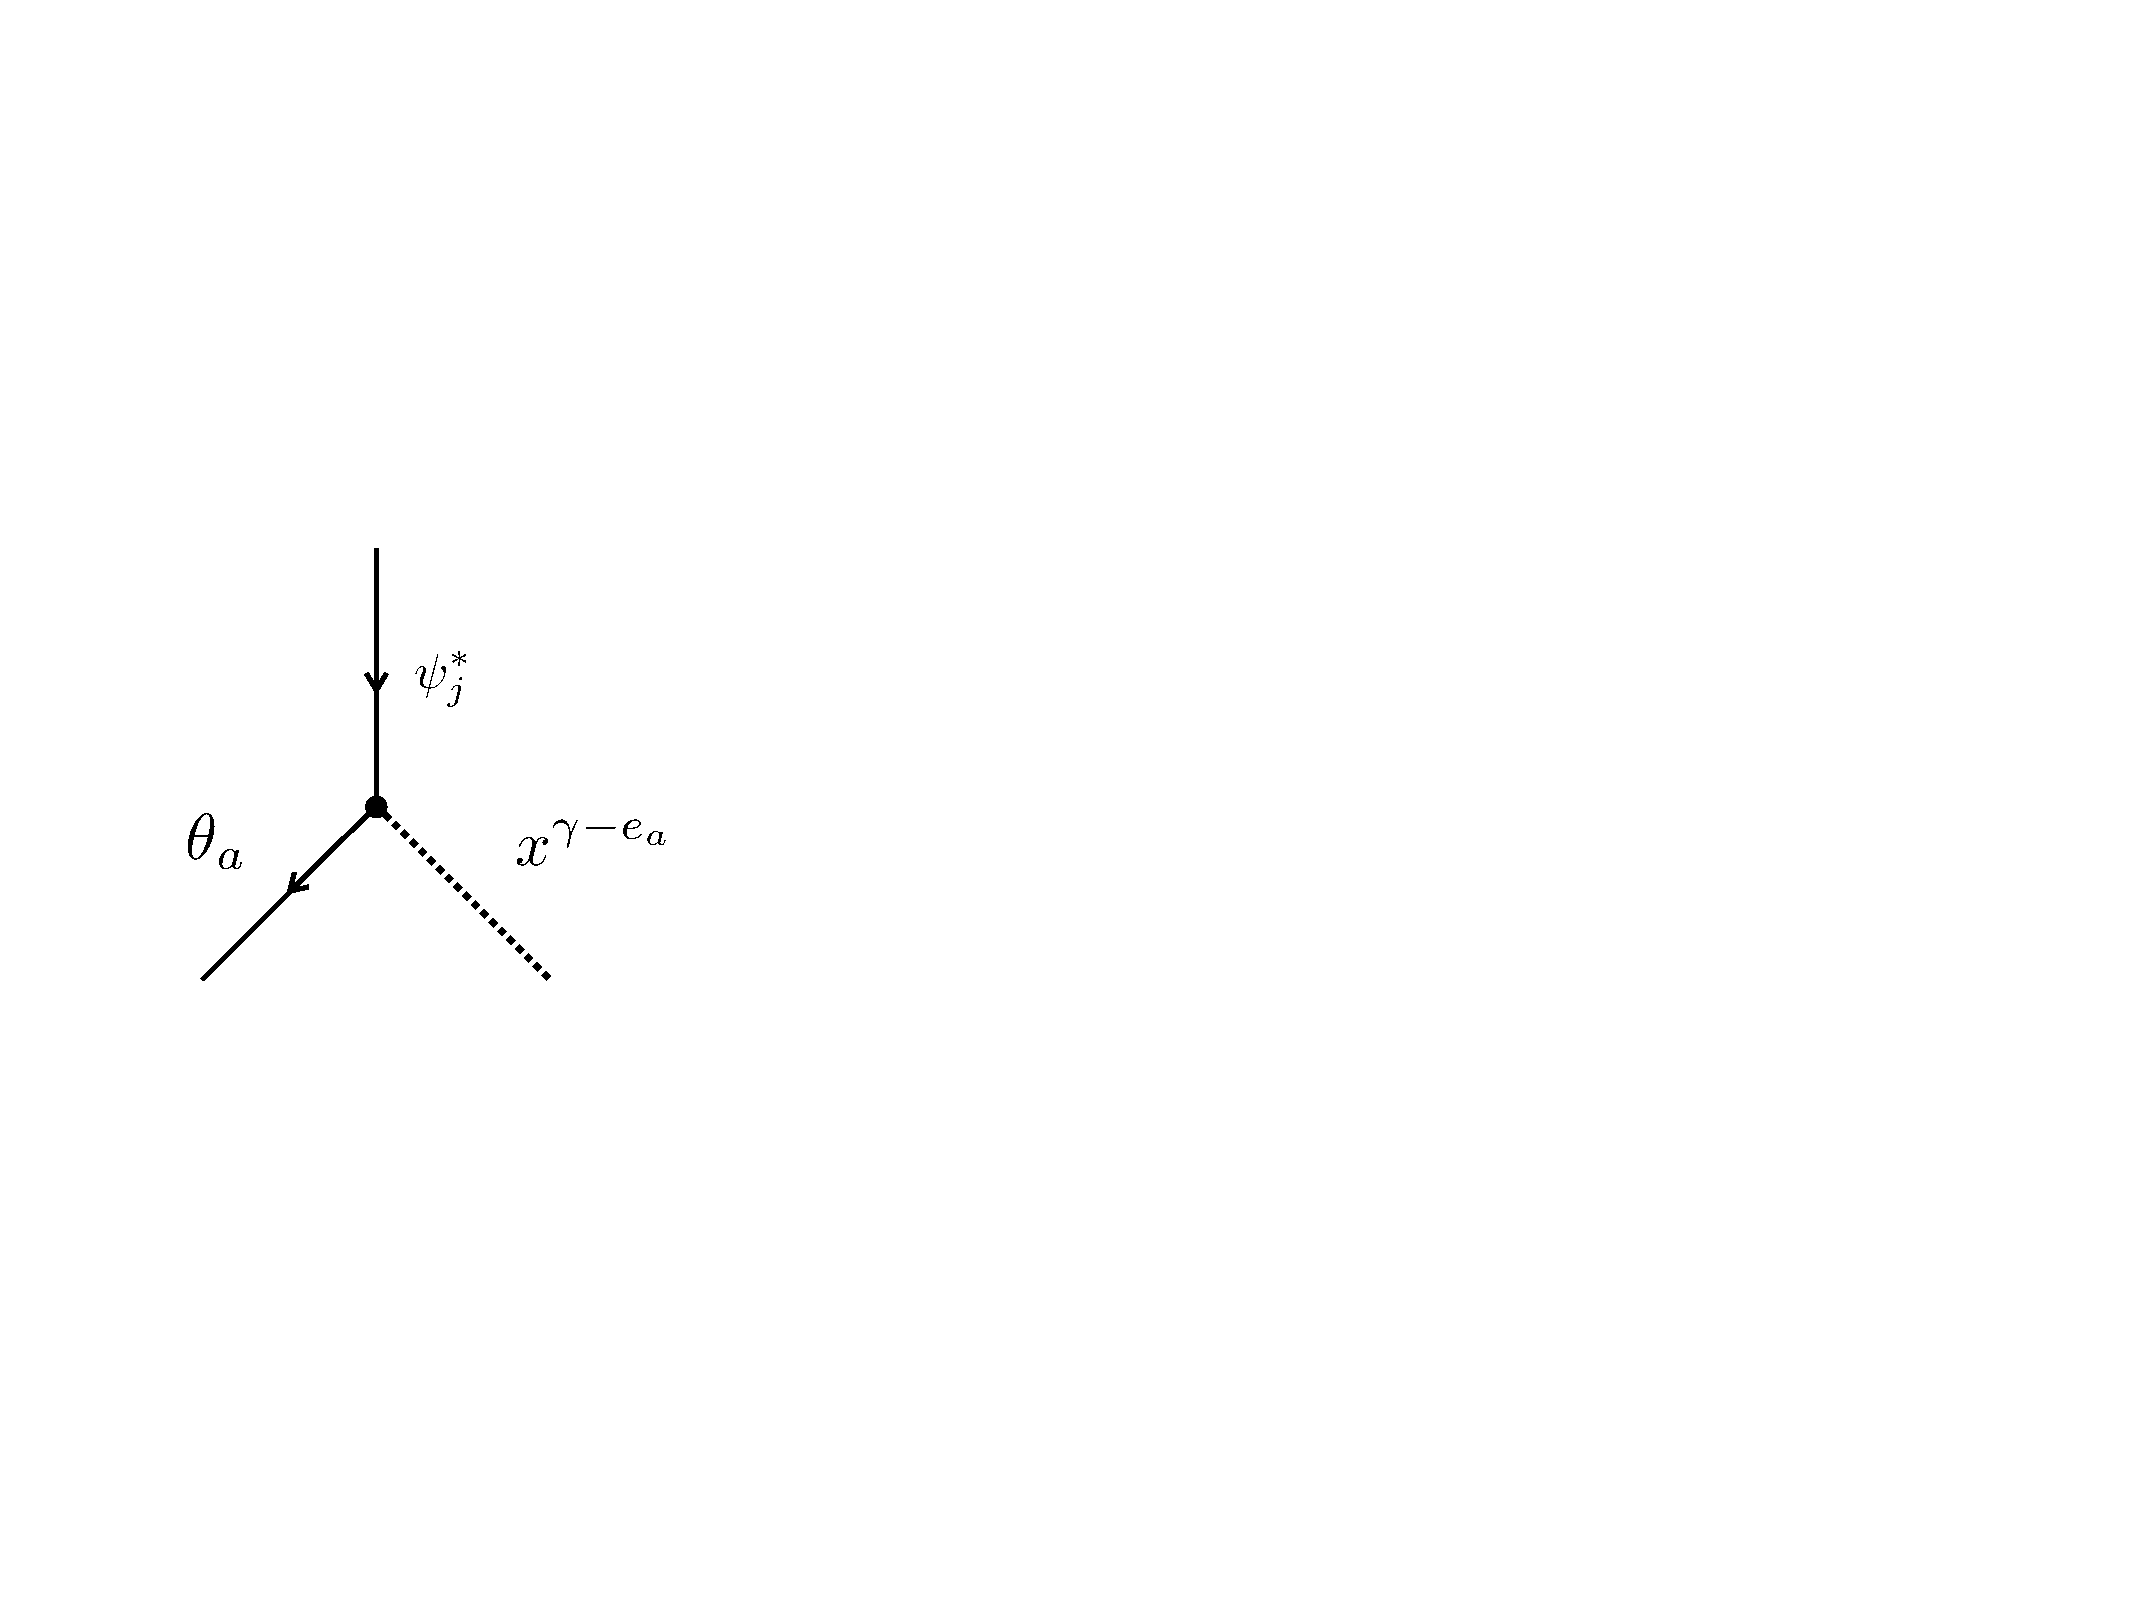
\includegraphics[scale=0.4]{dia2}
&
$\theta_a x^{\gamma - e_a} \big[\psi_j, -\big] \in \End_k( \mathscr{H} )$\\
\vspace{0.5cm}
$1 \le a,j \le n\,, \gamma \in \mathbb{N}^n$
&
\tagarray{\label{interaction_1}}
\end{tabular}
\end{center}

\begin{center}
\begin{tabular}{ >{\centering}m{1cm} >{\centering}m{4cm} >{\centering}m{8cm} >{\centering}m{1cm}}
\textbf{B}
&
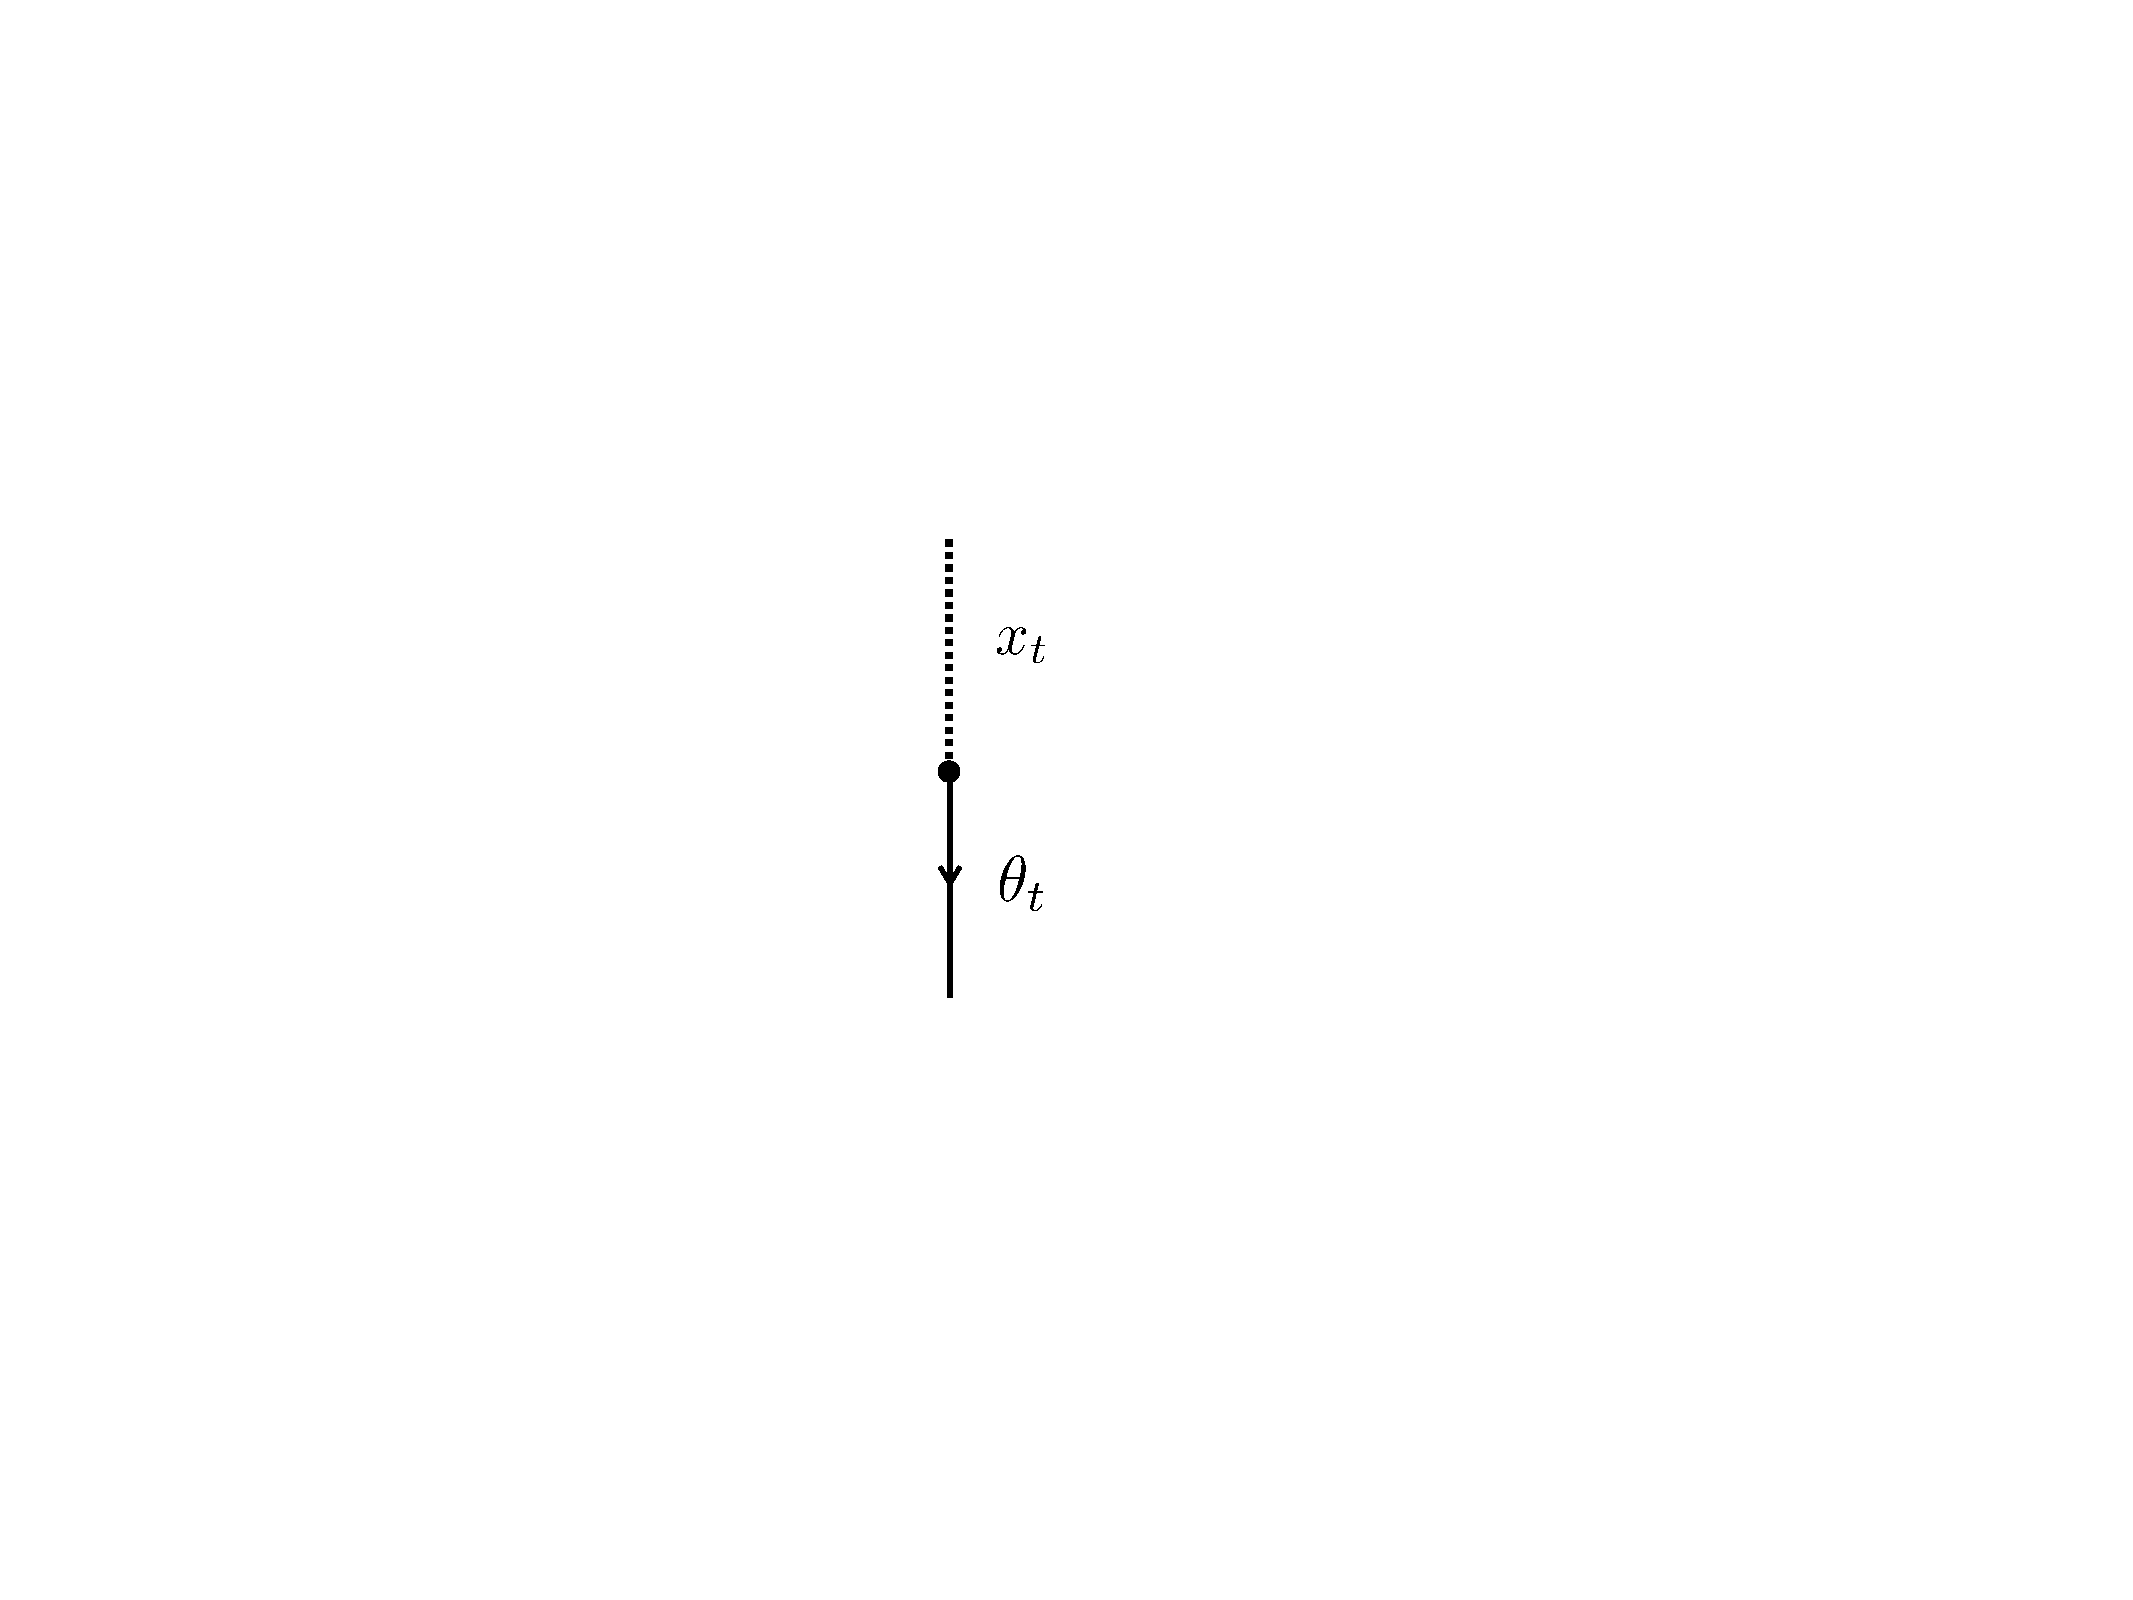
\includegraphics[scale=0.4]{dia3}
&
$\theta_t \partial_t \in \End_k( \mathscr{H} )$\\
\vspace{0.5cm}
$1 \le t \le n$
&
\tagarray{\label{interaction_2}}
\end{tabular}
\end{center}

\begin{center}
\begin{tabular}{ >{\centering}m{1cm} >{\centering}m{4cm} >{\centering}m{8cm} >{\centering}m{1cm}}
\textbf{C}
&
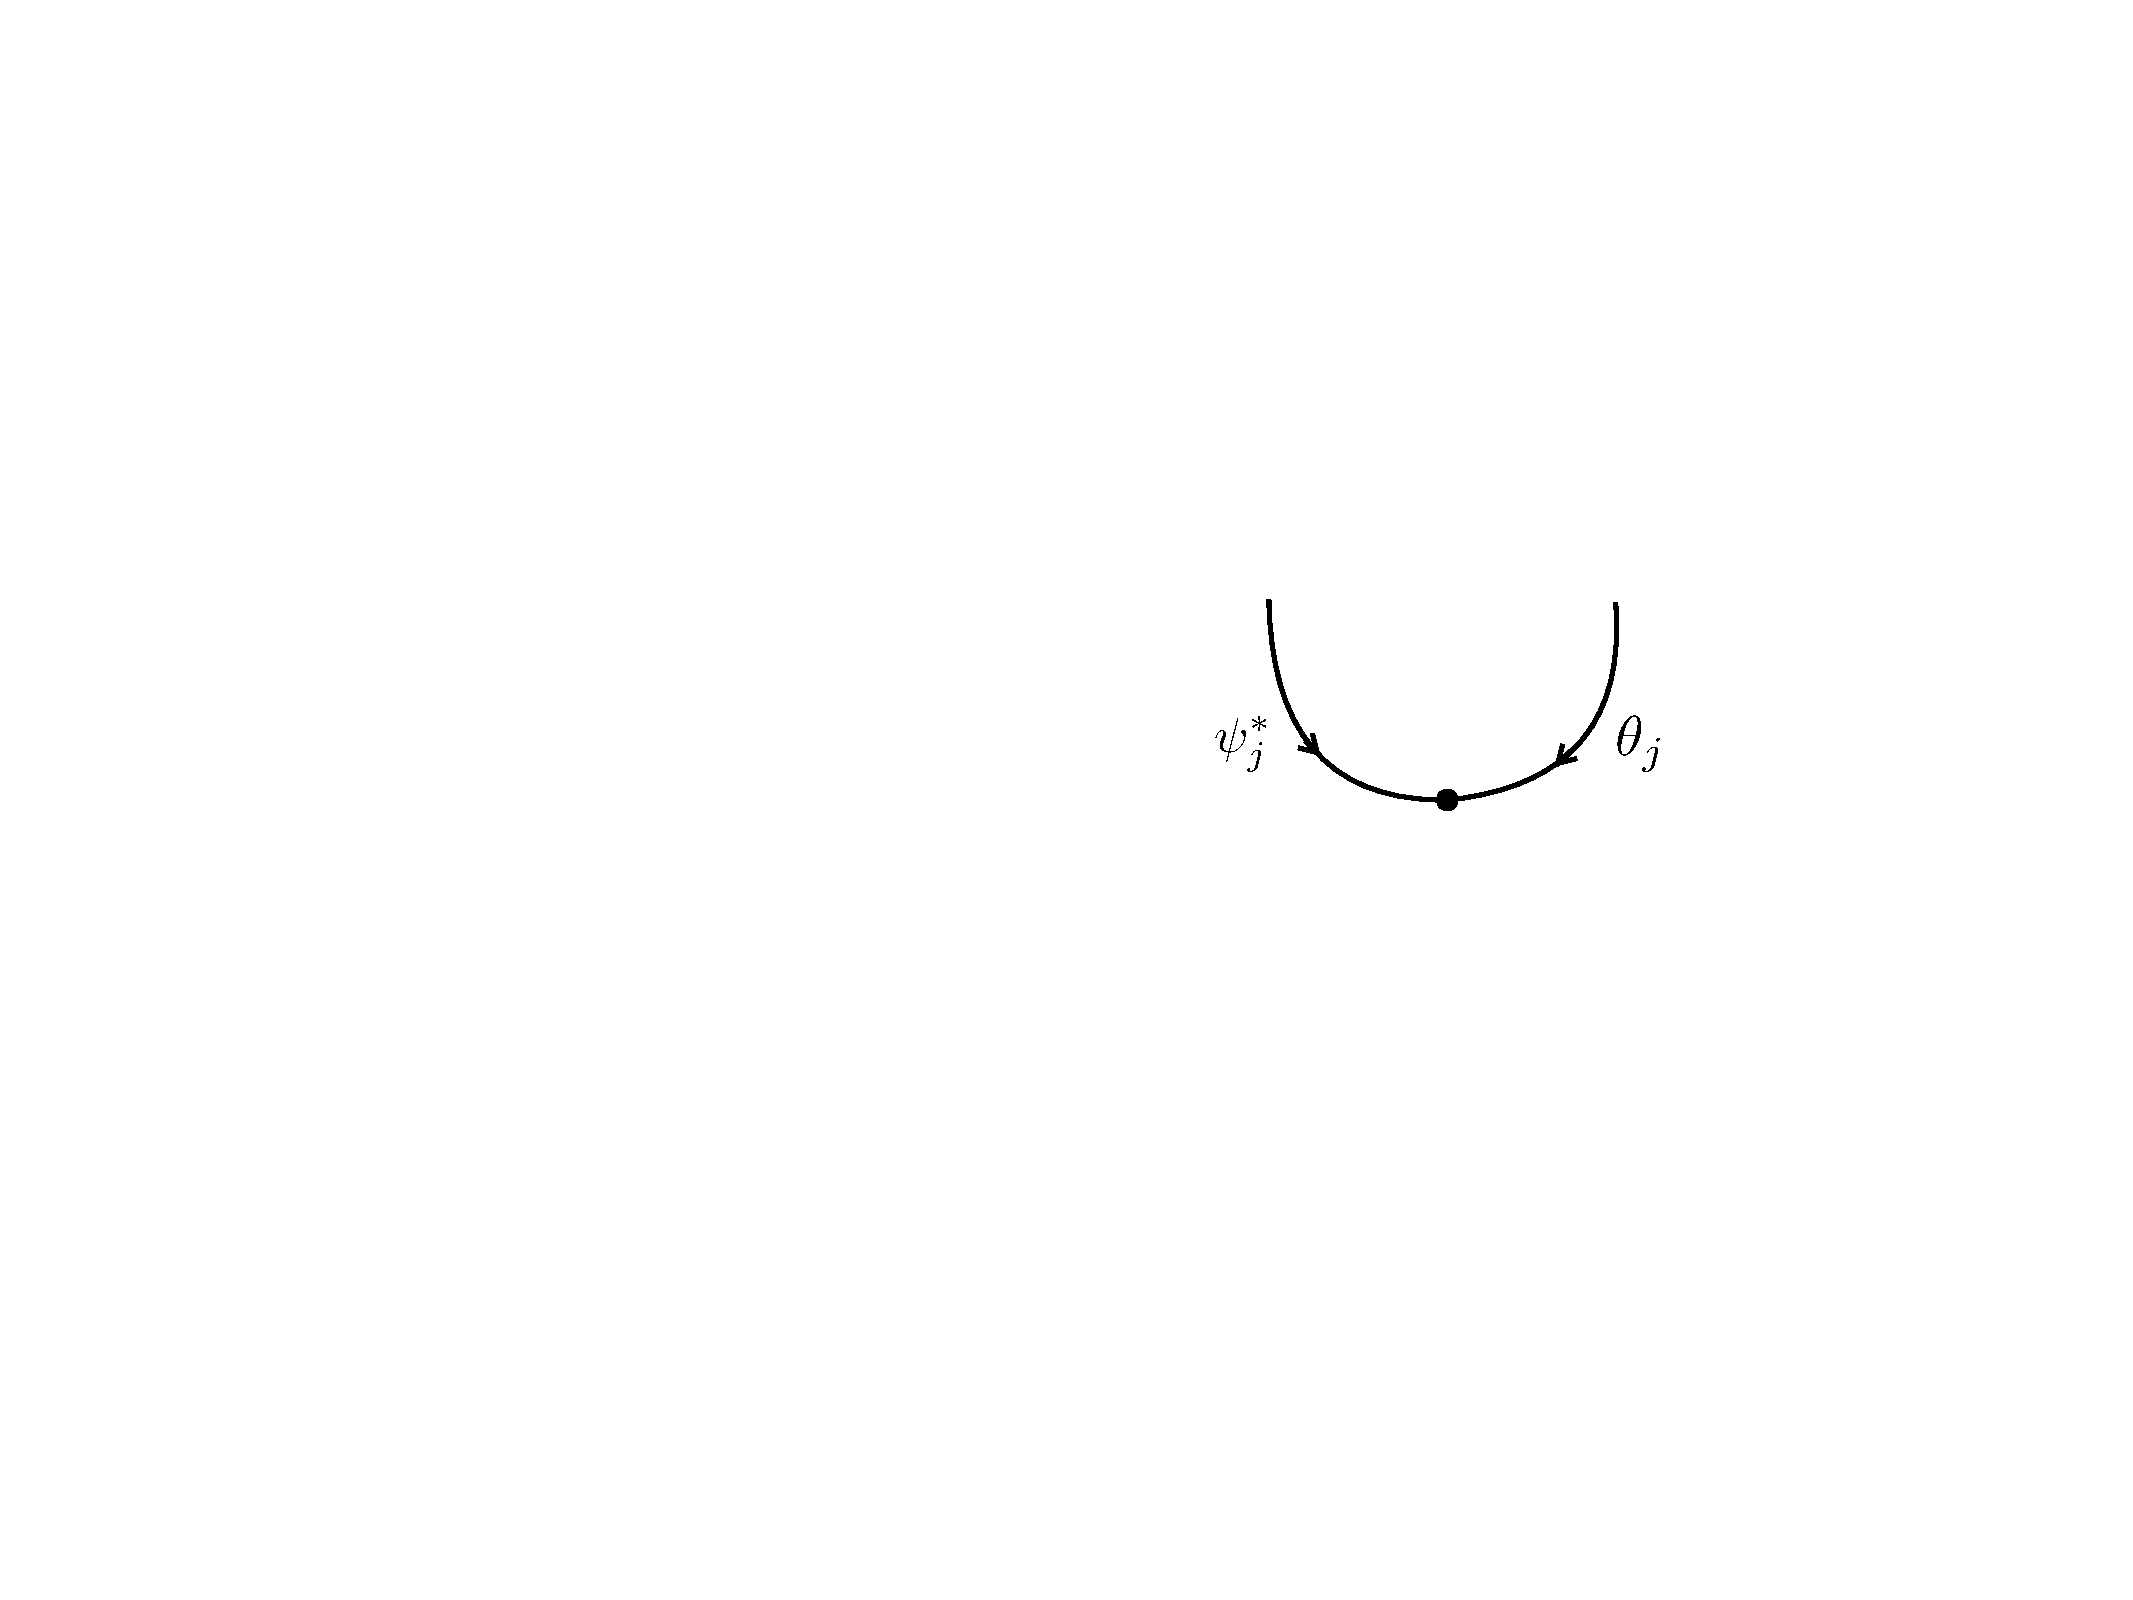
\includegraphics[scale=0.4]{dia4}
&
$m_2 \big( \big[\psi_j,-\big] \otimes \theta_j^* \big) \in \Hom_k( \mathscr{H}^{\otimes 2}, \mathscr{H} )$\\
\vspace{0.5cm}
$1 \le j \le n$
&
\tagarray{\label{interaction_3}}
\end{tabular}
\end{center}
Here $m_2$ is the multiplication in $\mathscr{H}$ and, given $\gamma \in \mathbb{N}^n$, we write $x^\gamma = x_1^{\gamma_1} \cdots x_n^{\gamma_n}$, with $e_i \in \mathbb{N}^n$ the unit vector with $x^{e_i} = x_i$. By convention if $\gamma_a = 0$ then $x^{\gamma - e_a} = 0$, which ensures that we always have $\gamma_a x^{\gamma - e_a} = \partial_a(x^\gamma)$. Finally note that bosons are depicted with dotted lines, and fermions with solid lines.

These interactions ``take place'' at vertices of the tree $A(T)$ for some $T \in \cat{T}_q$, and come with the following constraints, which will be formalised below in terms of combinatorial data called \emph{configurations}. We write $f(\gamma)$ for the coefficient of $x^\gamma$ in a polynomial $f \in R$ and recall the chosen decomposition $W = \sum_j x_j W^j$. 

\begin{itemize}
\item A-type interactions only occur at input vertices and internal edges of $T$. 
\item B-type interactions only occur at internal edges of $T$.
\item C-type interactions only occur at internal vertices of $T$, and moreover the incoming lines must come from different branches of the tree.
\item There may be arbitrarily many A-type or C-type interactions per vertex of $A(T)$, but there is \emph{precisely one} B-type interaction at each internal edge of $T$.
\item The A-type interaction with indices $a,j, \gamma$ appears with the coefficient
\be\label{eq:coeff_a}
-\frac{\gamma_a}{|\gamma|} W^j( \gamma)\,.
\ee
where $|\gamma| = \sum_{i=1}^n \gamma_i$. Each B- and C-type interaction appears with coefficient $(-1)$.
\end{itemize}

As we will see, the coefficient \eqref{eq:coeff_a} is the only way that $W$ enters the rules, and thus the definition of the $A_\infty$-products on $\mathscr{B}$. The precise definition of the Feynman rules will be given in Definition \ref{defn:config} below, but first we give an example of a tree with interactions inserted, to illustrate the various ingredients.

\begin{example}\label{ex:picture_example} Consider the tree $T \in \cat{T}_3$ whose augmented tree $A(T)$ is depicted below, together with labels for its vertices, where we label by $e$ the vertex corresponding to the internal edge of $T$:
\begin{center}
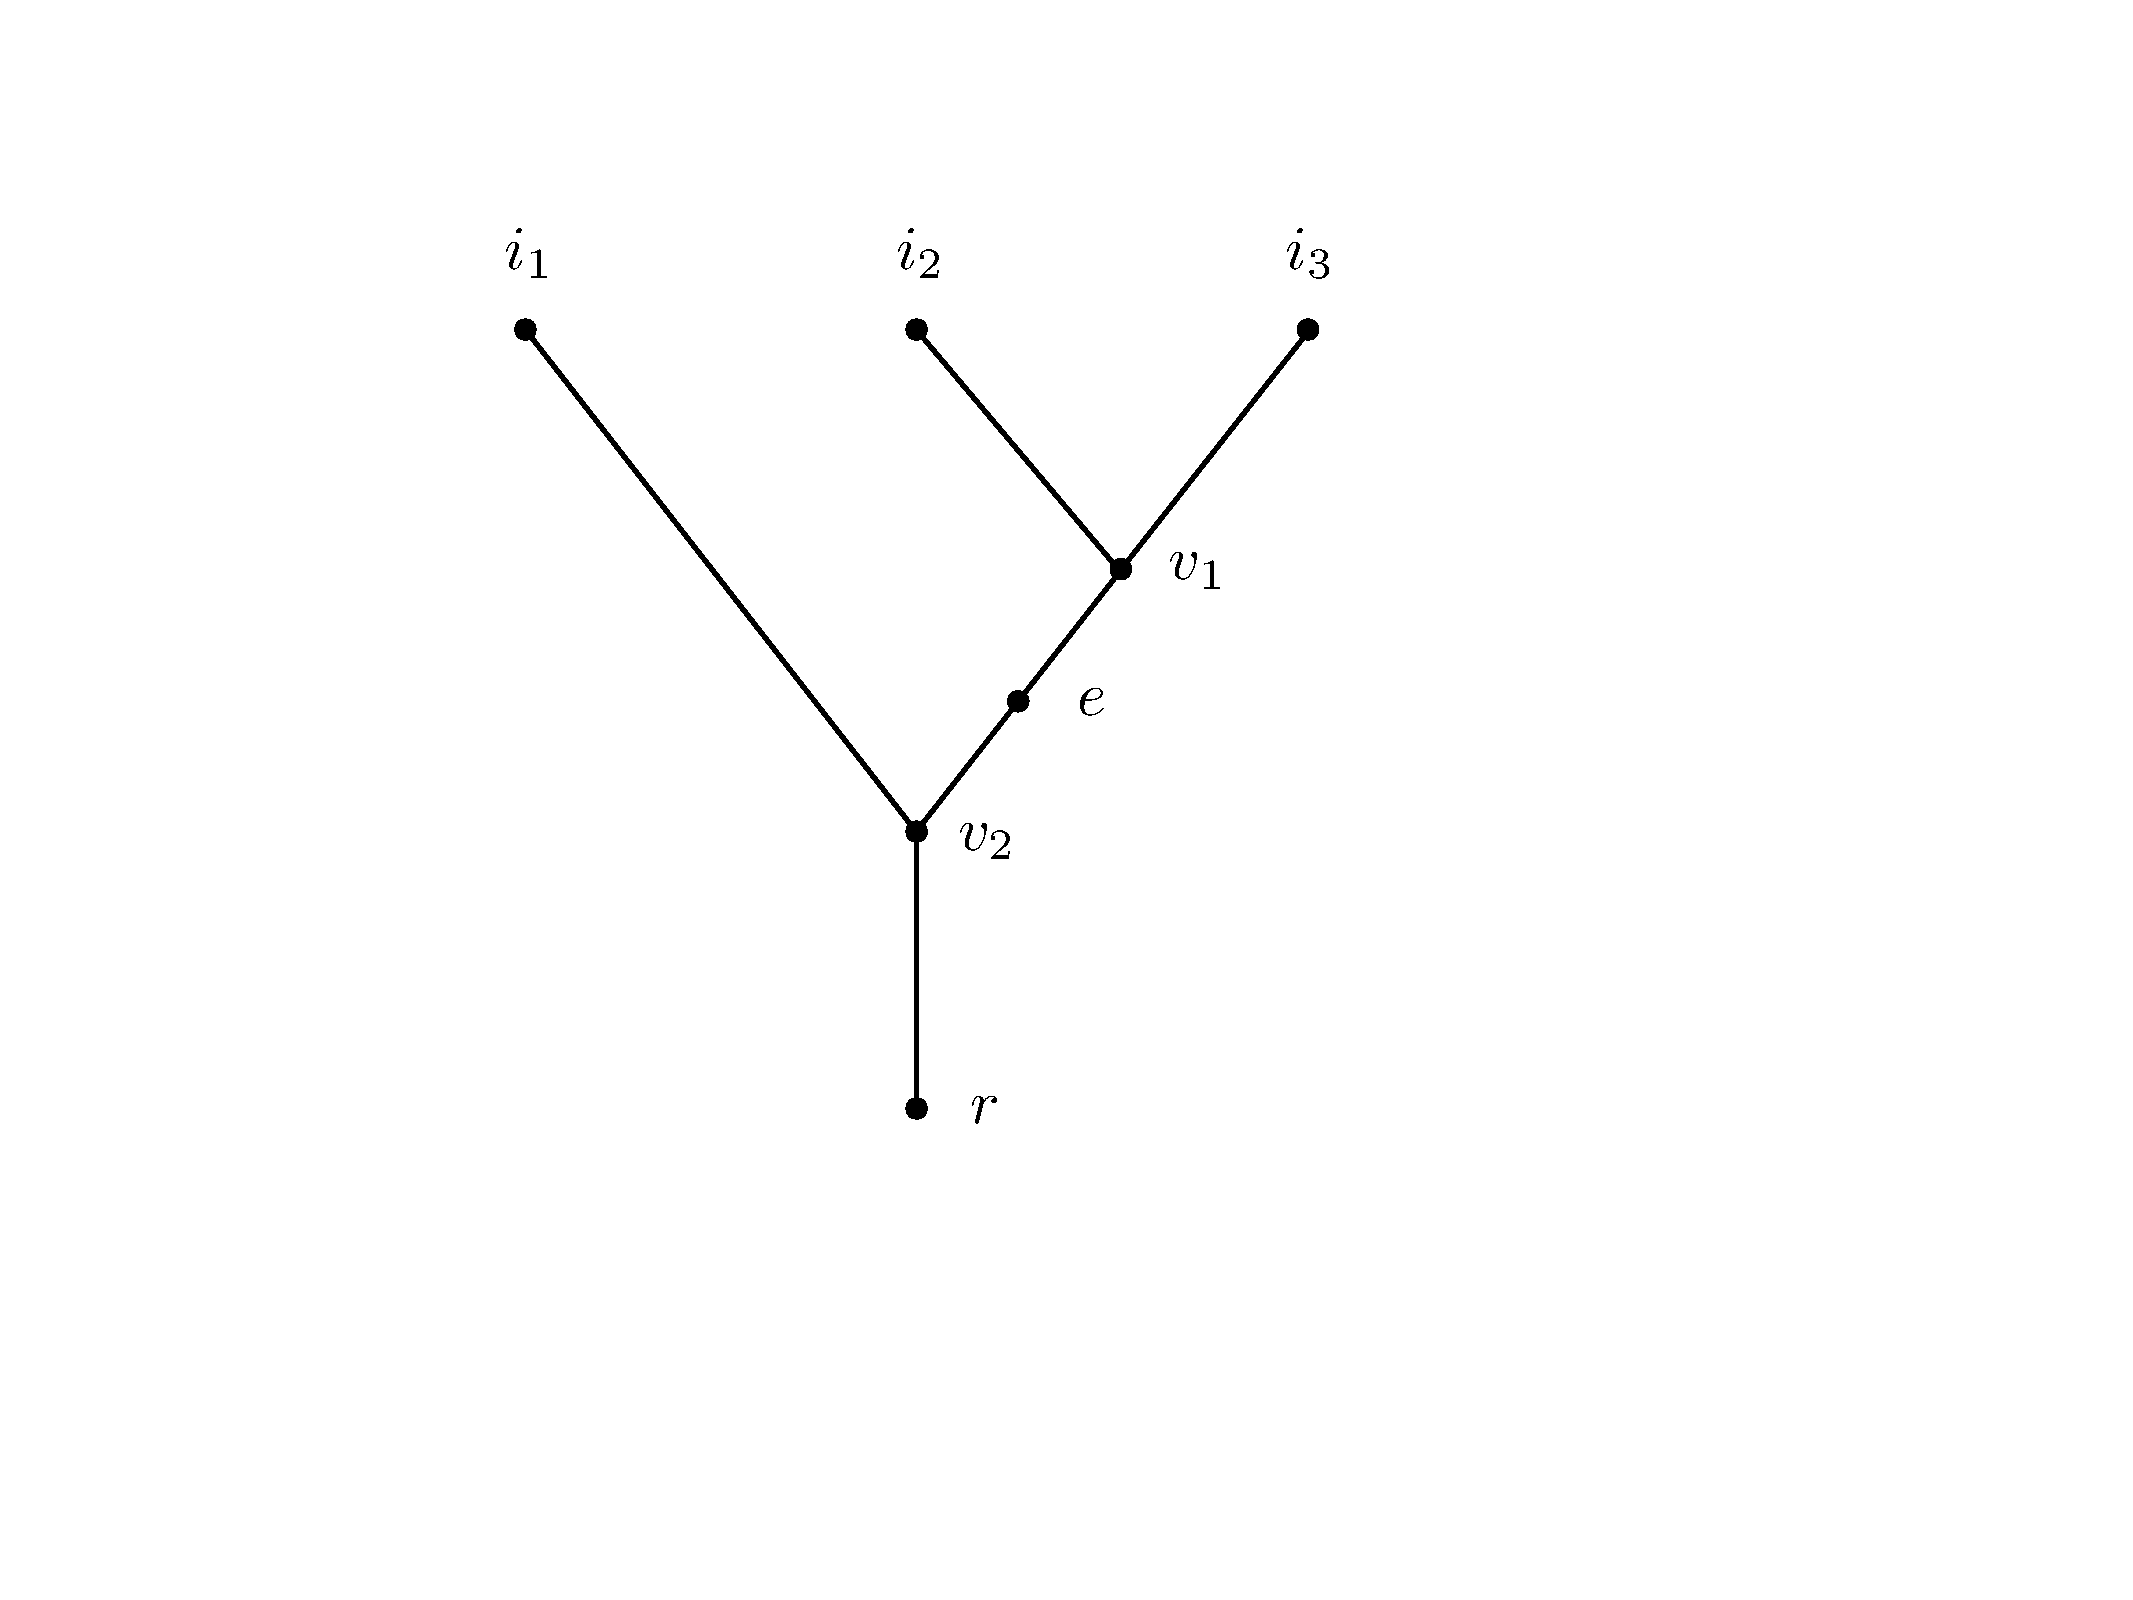
\includegraphics[scale=0.25]{dia7}
\end{center}
Set $W = x^3 \in \mathbb{C}[x]$ so that $W^1 = x^2$ and the only A-type interaction has $a = 1, j = 1, \gamma = 2$ and coefficient $-1$, as in the diagram (we write $\theta = \theta_1, \psi = \psi_1$)
\begin{center}
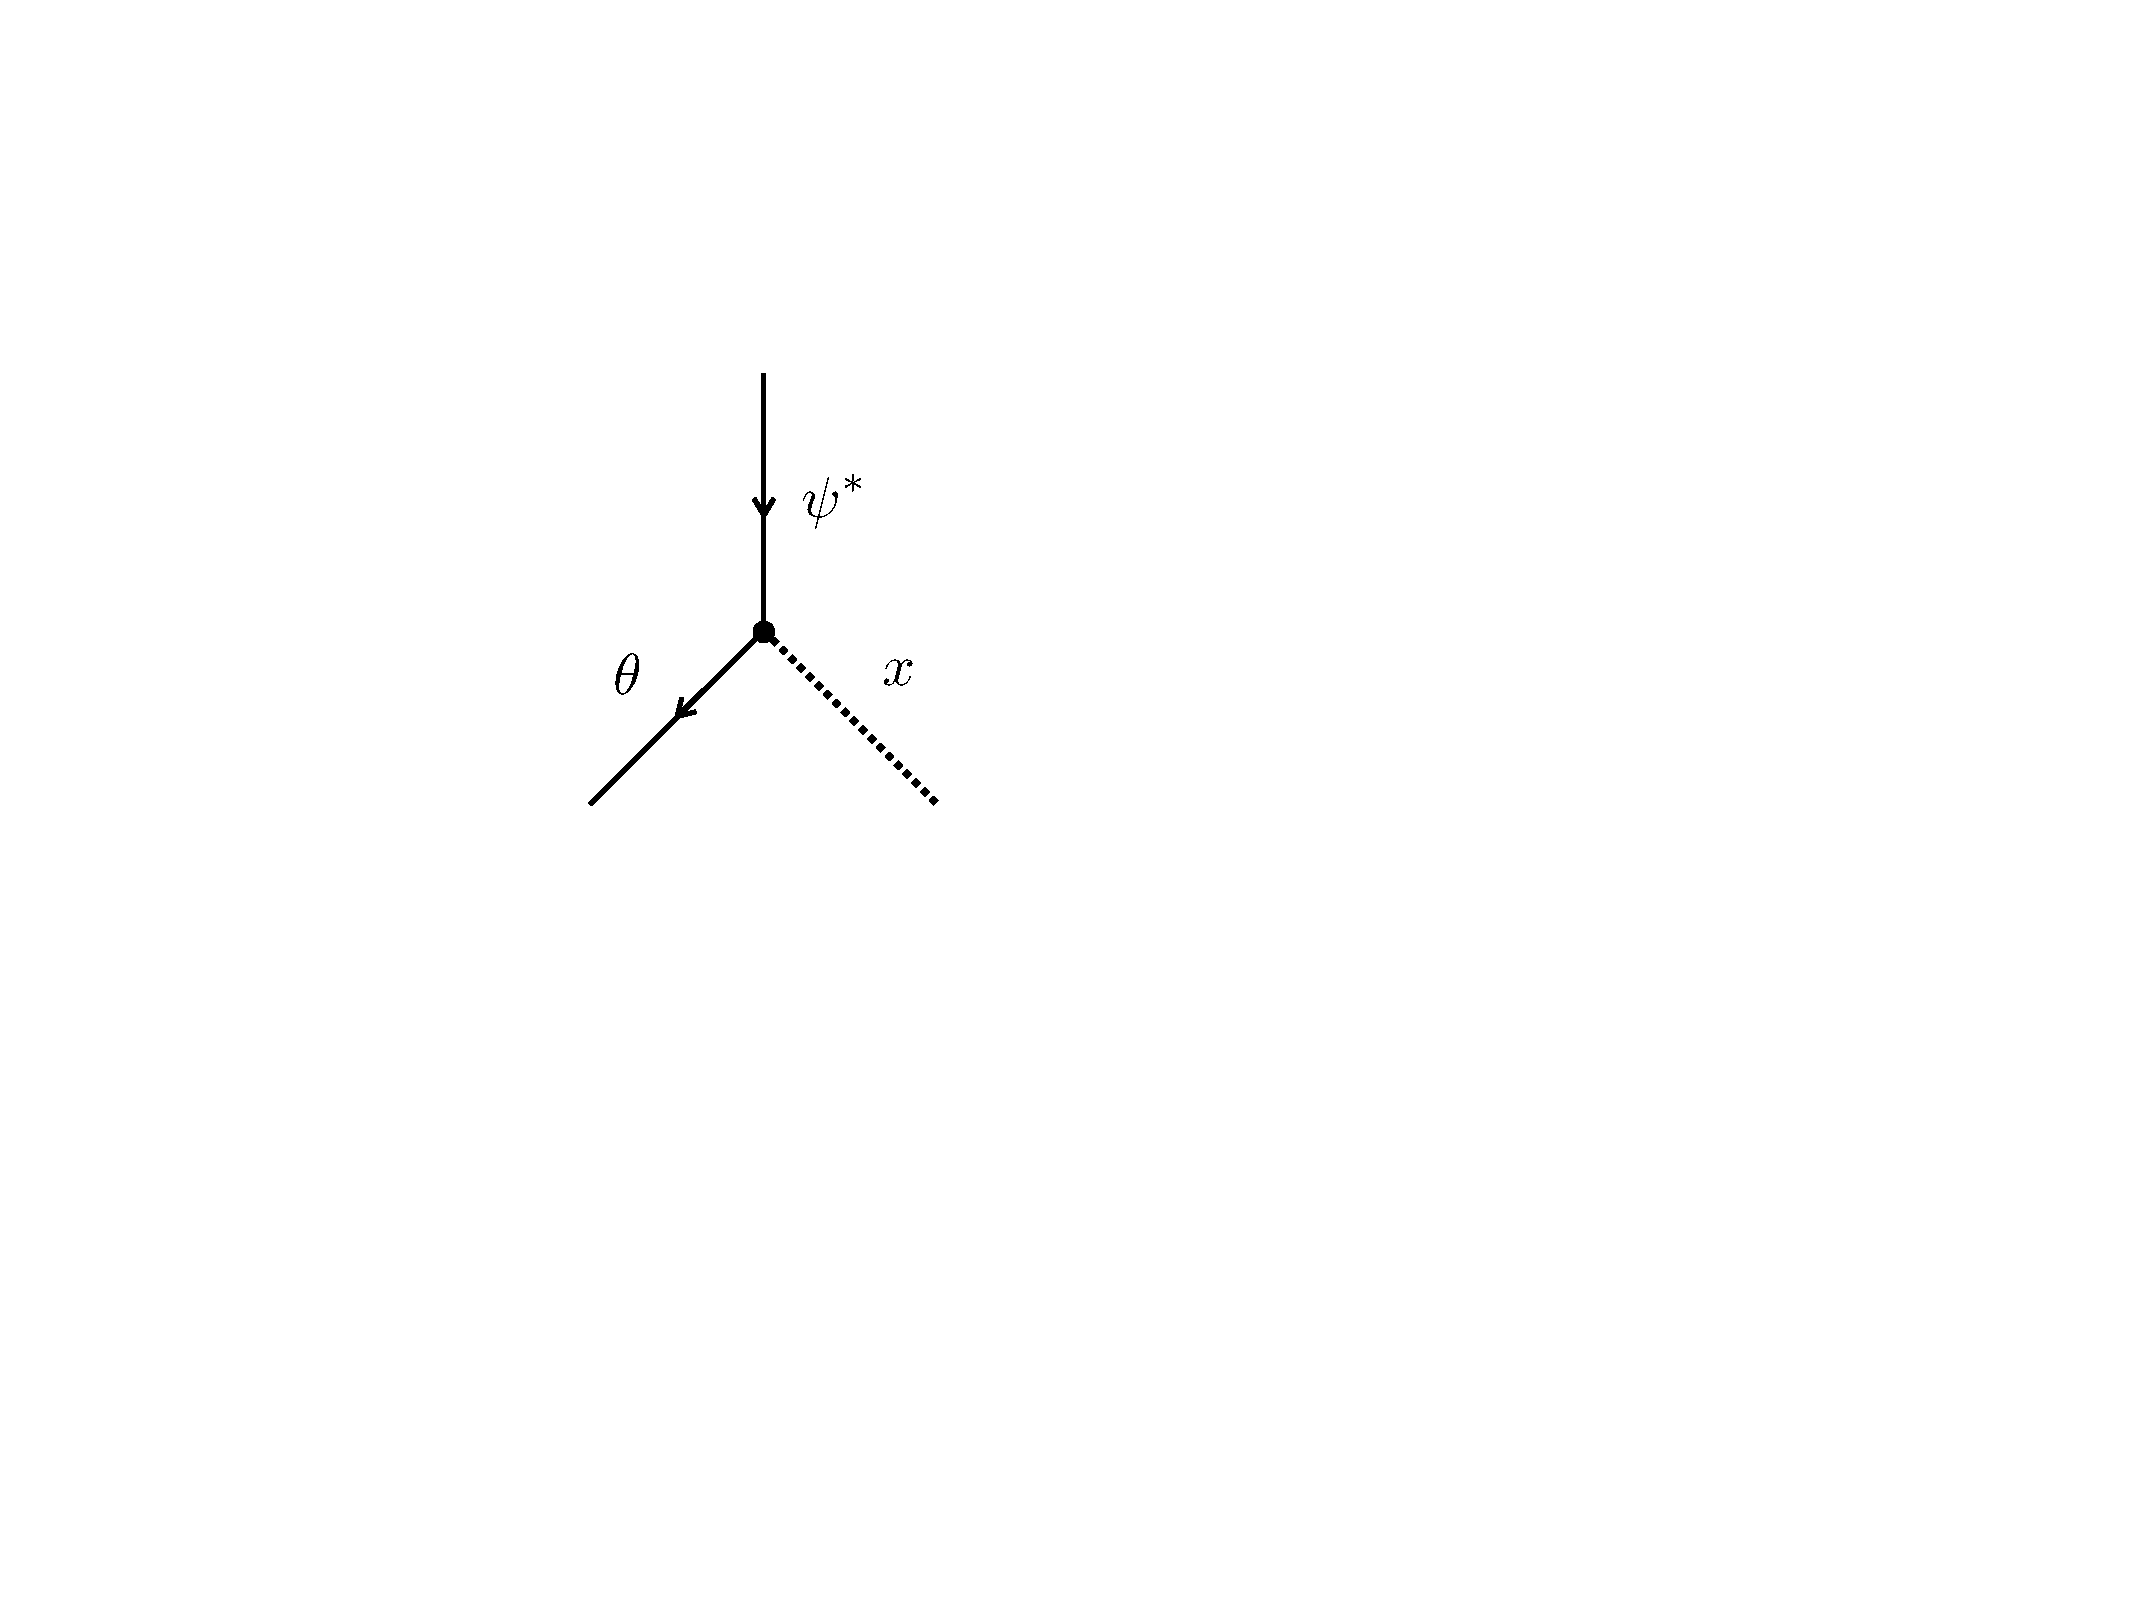
\includegraphics[scale=0.3]{dia5}
\end{center}
Consider the input state $\Psi = \psi^* \otimes \psi^* \otimes \psi^*$ in $\mathscr{B}^{\otimes 3}$. One possible pattern of interactions (called a configuration, below) has a single A-type interaction at the input vertex $i_3$, a B-type interaction at $e$, and two C-type interactions at $v_1,v_2$, as shown in the following ``topological'' Feynman diagram
\begin{center}
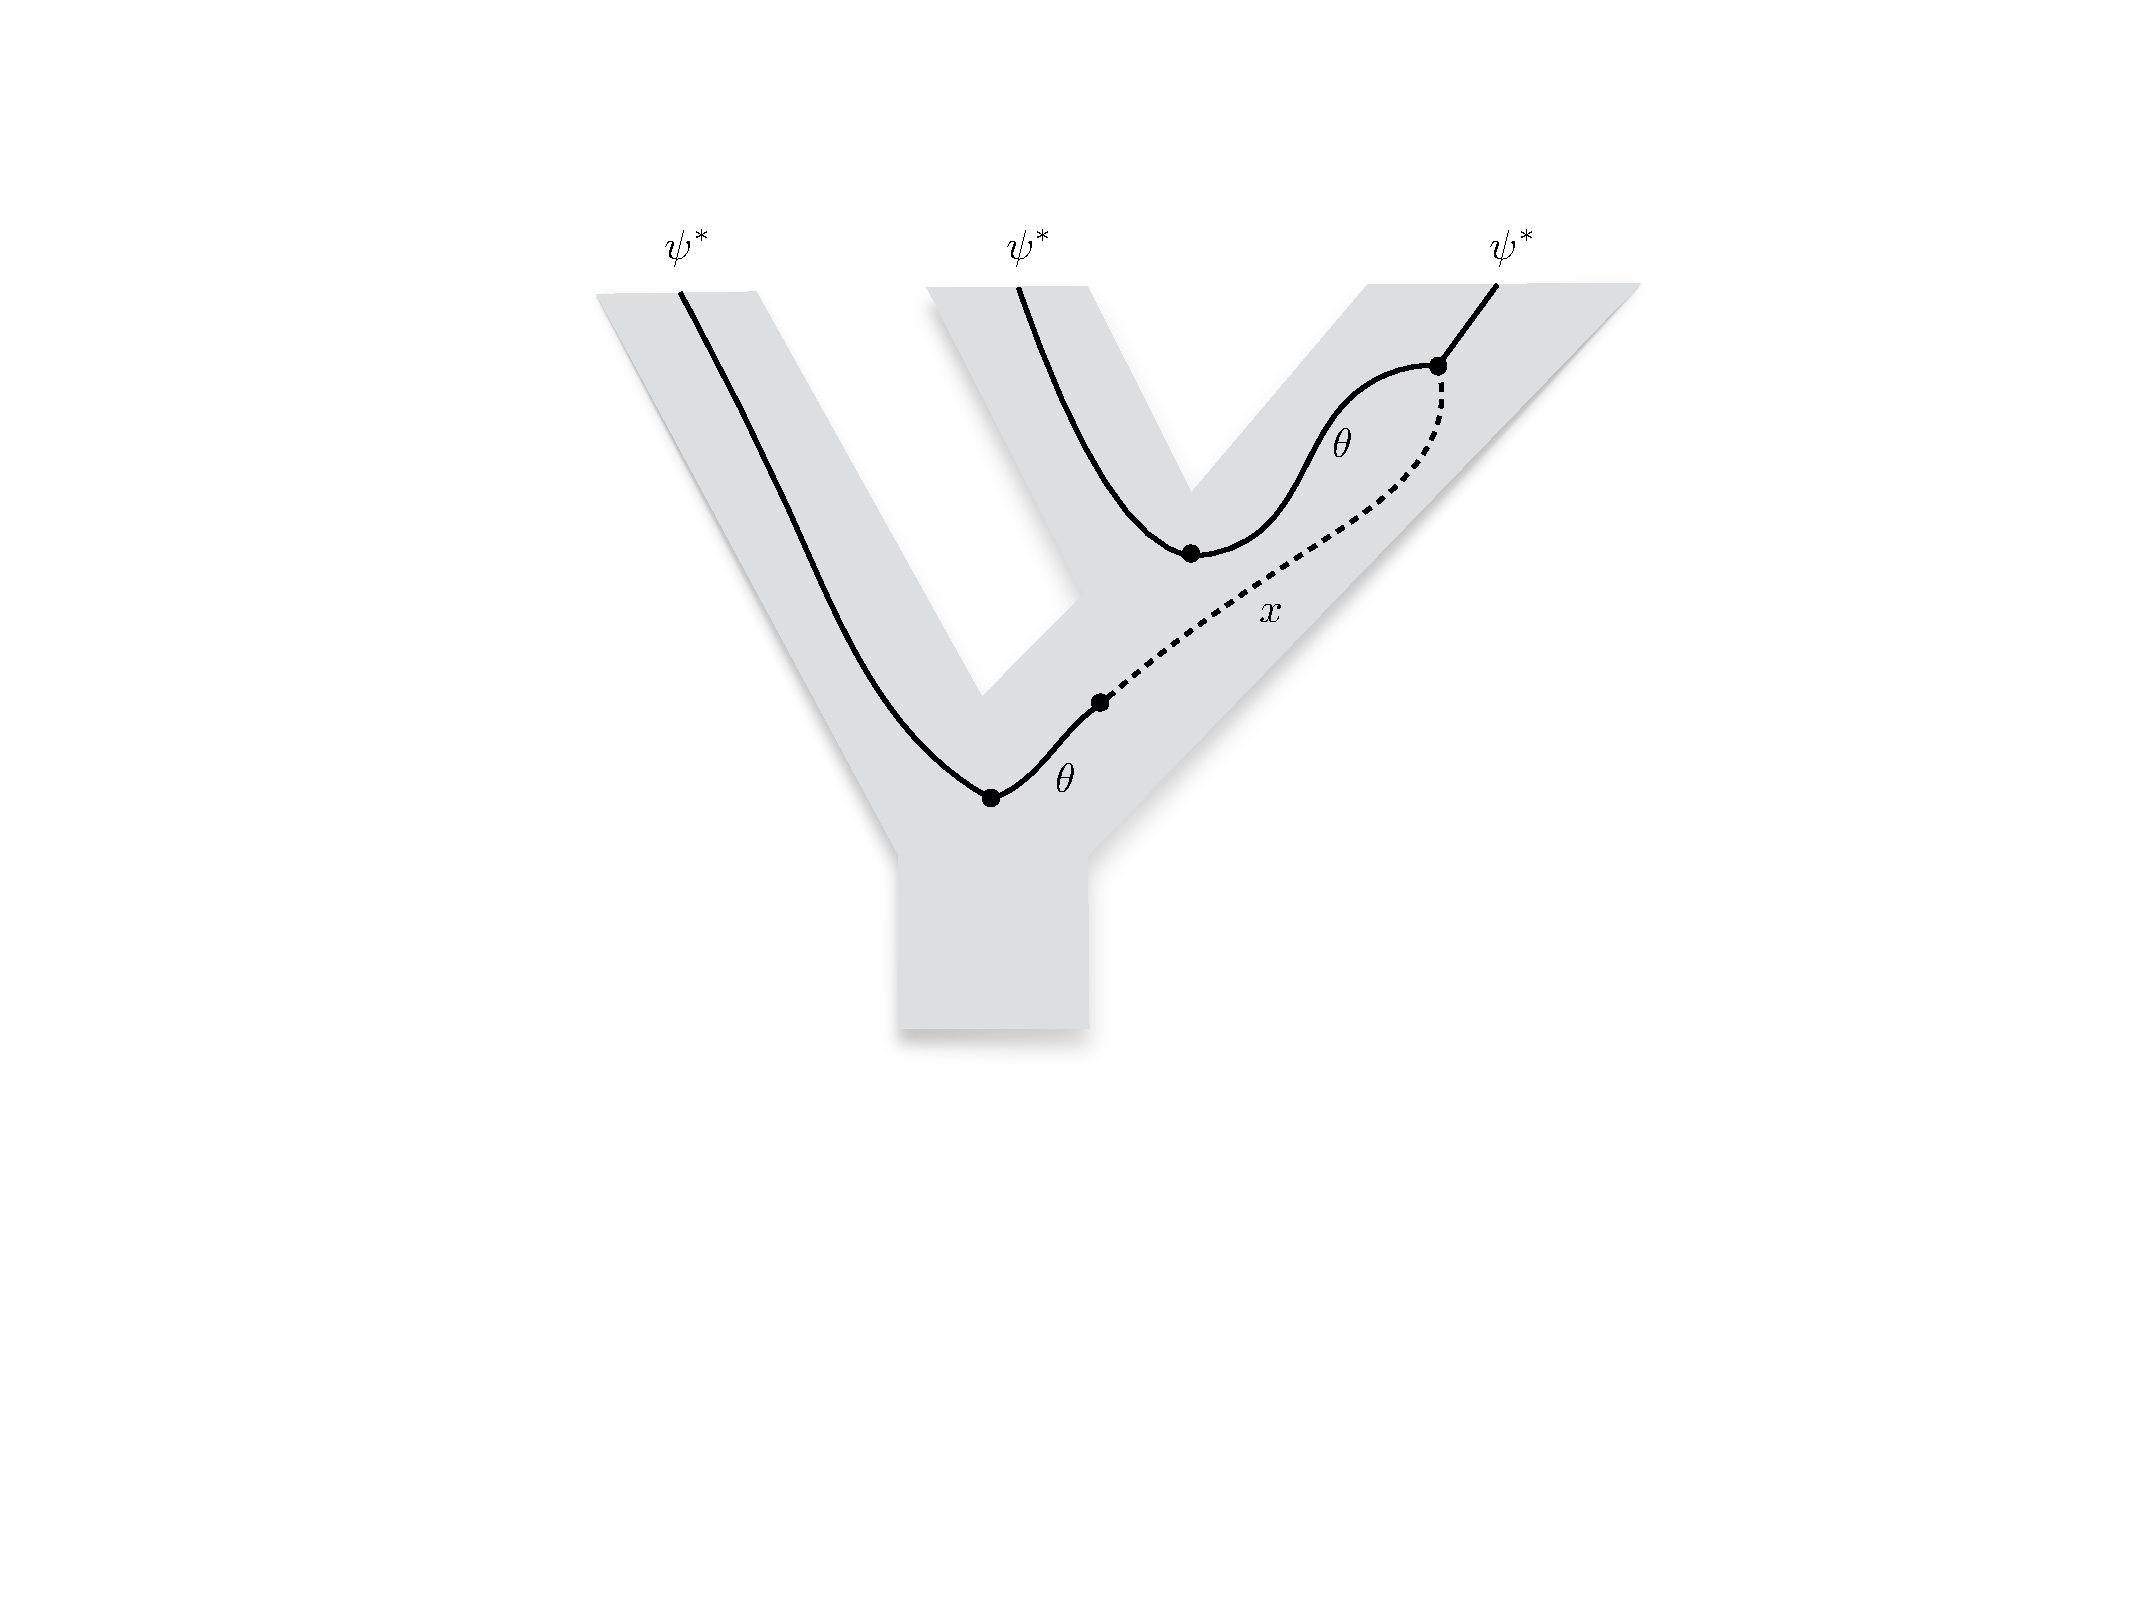
\includegraphics[scale=0.3]{dia6}
\end{center}
The \emph{value} of this diagram is the value of the linear map
\be\label{eq:operator_tree_example}
(-1)^3 p \circ m_2 \big([\psi, -] \otimes \theta^*\big) \circ \big( \sigma \otimes \theta \partial_x \circ m_2 ([\psi, -] \otimes \theta^*)\big( \sigma \otimes \theta x [\psi, -] \sigma \big)\big)
\ee
on the input state $\Psi$. Usually when evaluating such an expression we would pay attention to Koszul signs from commuting the input $\psi^*$'s into position (see Definition \ref{??}). Ignoring all signs, the value is
\begin{align*}
\pm \; & p \circ m_2 \big([\psi, -] \otimes \theta^*\big) \circ \big( \sigma \otimes \theta \partial_x \circ m_2 ([\psi, -] \otimes \theta^*)\big( \sigma \otimes \theta x [\psi, -] \sigma \big)\big)\Big( \Psi \Big)\\
&= \pm \; p \circ m_2 \big([\psi, \psi^*] \otimes \theta^* \theta \partial_x \circ m_2 ([\psi, \psi^*] \otimes \theta^* \theta x [\psi, \psi^*] \big)\big)\\
&= \pm \; p \circ m_2 \big(1 \otimes \theta^* \theta \partial_x \circ m_2 (1 \otimes \theta^* \theta x \big)\big)\\
&= \pm \; p \circ m_2 \big(1 \otimes \partial_x(x) \big)\\
&= \pm \; p(1) = \pm \; 1 \in \mathscr{H}\,.
\end{align*}
\end{example}

Now we give some more precise definitions. Let $T \in \cat{T}_q$ be a valid plane tree with $q$ inputs and $e_i(T)$ internal edges, and let $A(T)$ be the augmented plane tree. The definitions are all relative to the ambient integer $n$, but for the sake of readability we will not reflect this in the notation.

\begin{definition}\label{defn:config} A \emph{configuration} $C$ of a valid plane tree $T$ consists of the following data, for each non-root vertex $v$ of $A(T)$:
\begin{itemize}
\item An integer $m(v) \ge 0$.
\item A subset $J(v) \subseteq \{ 1,\ldots, n \}$ with $|J(v)| = m(v)$. 
\item If $v$ is an input, or comes from an internal edge of $T$, a pair
\[
( a_j(v), \gamma_j(v) ) \in \{ 1, \ldots, n \} \times \mathbb{N}^n
\]
for each $j \in J(v)$, with $\gamma_j(v)_{a_j(v)} \ge 1$.
\item If $v$ comes from an internal edge of $T$, an integer $t(v) \in \{1,\ldots,n\}$.
\end{itemize}
Let $\operatorname{Con}(T)$ denote the set of all configurations.
\end{definition} 

\begin{remark}\label{remark:config_count} The integer $m(v)$ counts how many interactions of type A or C take place at $v$ (there is no point counting B interactions as precisely one occurs at each internal edge). The set $J(v)$ consists of all $j$-indices appearing in interactions at $v$. The interactions of A-type (at inputs and internal edges) are defined by indices $a_j(v), \gamma_j(v)$ while at each internal edge $e$ of $T$, $t(e)$ is the index of the B-type interaction.

Note that a configuration may contain no A-type or C-type interactions, that is, we may have $m(v) = 0$ for every non-root vertex $v$ of $A(T)$. Then the configuration is just the assignment of an integer $1 \le t(e) \le n$ to every internal edge $e$ of $T$. For the unique tree $T \in \cat{T}_2$ with two inputs, there are no internal edges and precisely one configuration with $m(v) = 0$ for all $v$.
\end{remark}

\begin{definition} Given a tree $T \in \cat{T}_q$ and configuration $C \in \operatorname{Con}(T)$ we define a decoration $D_{T,C}$ of $A(T)$ by the assignment of the modules
\begin{itemize}
\item $\mathscr{B}$ to the input at each non-root leaf, and
\item $\mathscr{H}$ to each edge and the output at the root.
\end{itemize}
To each vertex $v$ of $A(T)$ we associate an operator $\phi_v$ as follows, writing $m, J, \{ (a_j, \gamma_j) \}_{j \in J}, t$ for the data associated to $v$ by the configuration $C$:
\begin{itemize}
\item if $v$ is an input, then $\phi_v$ is the linear map $\mathscr{B} \lto \mathscr{H}$ given by
\be\label{eq:int_input}
\phi_v = (-1)^m \prod_{j \in J}\Big\{ \frac{1}{|\gamma_j|}(\gamma_j)_{a_j} W^j( \gamma_j)  \theta_{a_j} x^{\gamma_j - e_{a_j}} \big[ \psi_j, - \big] \Big\} \circ \sigma\,.
\ee
Note that the operator under the product is even, so the order is irrelevant. If $J(v)$ is empty then the product is interpreted to be the identity operator.
\item if $v$ comes from an internal edge of $T$, then
\be\label{eq:int_intedge}
\phi_v = (-1)^m \prod_{j \in J} \Big\{ \frac{1}{|\gamma_j|}(\gamma_j)_{a_j} W^j( \gamma_j)  \theta_{a_j} x^{\gamma_j - e_{a_j}} \big[ \psi_j, - \big] \Big\} \circ \theta_t \partial_t\,.
\ee
\item if $v$ comes from an internal vertex of $T$, then
\be\label{eq:int_intvert}
\phi_v = (-1)^m m_2 \circ \prod_{j \in J} \Big\{ \big[ \psi_j, - \big] \otimes \theta_j^* \Big\}
\ee
which is a map $\mathscr{H}^{\otimes 2} \lto \mathscr{H}$. Here $m_2$ denotes the product on $\mathscr{H}$.
\item if $v = r$ is the root, $\phi_v = p: \mathscr{H} \lto \mathscr{H}$ is the projection of Definition \ref{defn:handop}.
\end{itemize}
\end{definition}

The denotation $\langle D_{T,C} \rangle$ of this decoration is \emph{a priori} a linear map $\mathscr{B}^{\otimes q} \lto \mathscr{H}$, but since the only operators in the decoration acting on the third tensor factor of $\mathscr{H}$ in \eqref{eq:defn_H_space} are the commutators $[\psi_i,-]$ under which $\mathscr{B}$ is closed, $\langle D_{T,C} \rangle$ actually has its image contained in the submodule $\mathscr{B} \subseteq \mathscr{H}$. 

\begin{definition}\label{defn:otc} Given $T \in \cat{T}_q$ and $C \in \operatorname{Con}(T)$ we define the $k$-linear operator
\[
\cat{O}(T, C): \mathscr{B}^{\otimes q} \lto \mathscr{B}
\]
to be the denotation $\cat{O}(T,C) = \langle D_{T,C} \rangle$, defined without Koszul signs.
\end{definition}

\begin{example}\label{ex:picture_example_2} The configuration $C$ which is described in Example \ref{ex:picture_example} has $n = 1$ and
\begin{gather*}
m(i_3) = m(v_1) = m(v_2) = 1\,,\\
J(i_3) = J(v_1) = J(v_2) = \{ 1 \}\,,\\
t(e) = 1\,.
\end{gather*}
At $i_3$ we have the pair $a = 1$ and $x^\gamma = x^2$. The operator $\cat{O}(T,C)$ is precisely \eqref{eq:operator_tree_example}.
\end{example}

\begin{remark} Let us now briefly explain the connection between configurations, the linear map $\cat{O}(T,C)$ and Feynman diagrams, such as the one in Example \ref{ex:picture_example}. Ultimately we will not actually use these diagrams to perform calculations, so we refrain from formulating them too precisely; however, they are very useful as a tool for understanding.

We view $\Psi_1 \otimes \cdots \otimes \Psi_q \in \mathscr{B}^{\otimes q}$ as the result of applying creation operators (meaning wedge products $\psi_i^* \wedge -$) to the vacuum (meaning the identity of the exterior algebra) in the various copies of $\mathscr{B}$. The value of $\cat{O}(T,C)$ on $\Psi$ may be computed by commuting all creation operators acting on $\mathscr{H}$ (that is, the operators $x_i, \theta_i, \psi_i^*$) leftward in the expression, which means \emph{down} the tree. These operators commute with all other creation operators and with those annihilation operators that are either of a different type (e.g. $[x_i, \theta_j^*] = 0$) or of same type but with different indices (e.g. $[x_1, \partial_2] = 0$). However, there will be a nonzero commutator every time a creation operator meets an annihilation operator of the same type and index (respectively $\partial_i, \theta_i^*, [\psi_i, -]$). We view such a commutator, say
\[
\theta_i \theta_i^* + \theta_i^* \theta_i = [ \theta_i, \theta_i^* ] = 1\,,
\]
which arises as the result of commuting the $\theta_i$ leftward to meet the $\theta_i^*$, as generating two diagrams, corresponding to the two choices of summands in $\theta_i^* \theta_i = 1 - \theta_i \theta_i^*$. Choosing the first summand means there is an interaction (drawn as a line marked $\theta_i$ from the original position of the $\theta_i$ to the position of the $\theta_i^*$ in the tree) while choosing the second summand means there is no interaction (the $\theta_i$ sails on, to meet its partner further down the tree). If a particular series of choices leads to an $x_i$ or $\theta_i$ meeting the bottom of the tree then this diagram does not contribute to $\cat{O}(T,C)(\Psi)$ since $p$ projects out such elements of $\mathscr{H}$. 

We can depict a series of choices by linking the creation and annihilation operators,
\begin{center}
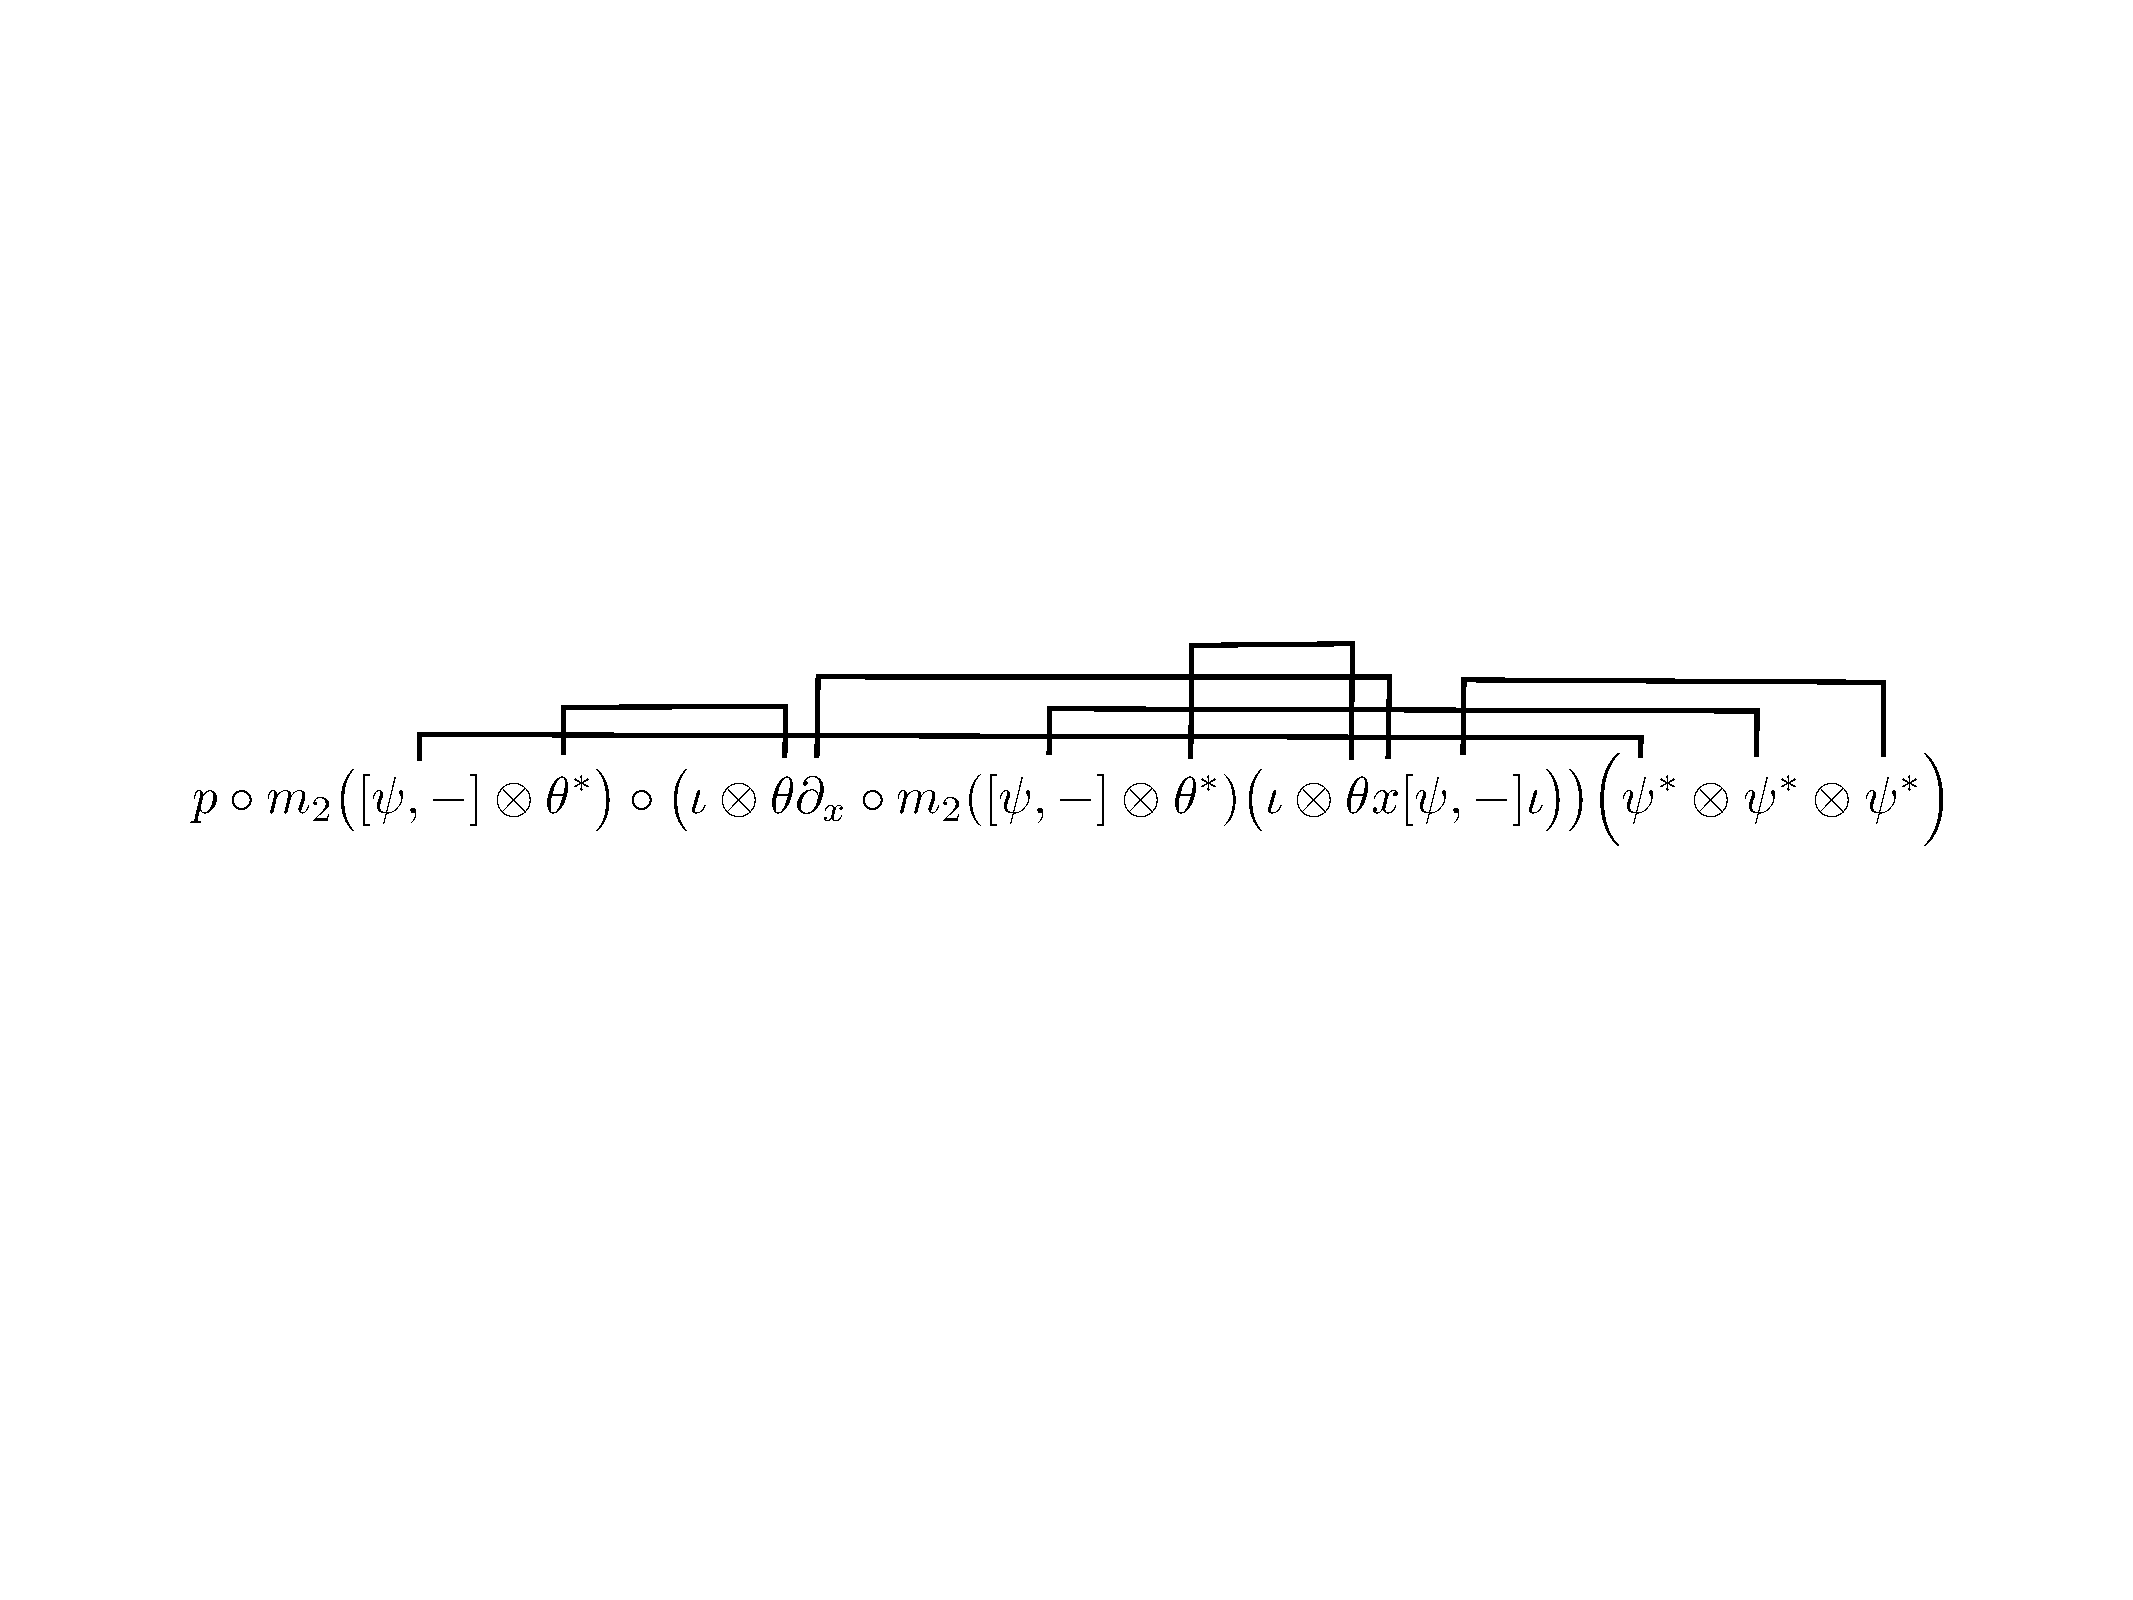
\includegraphics[scale=0.45]{dia8}
\end{center}
or by drawing these linkages, marked with the type and index of the ``particle'' on the tree $T$, joining the two positions determined by the configuration as in Example \ref{ex:picture_example}.

Note that in this example one of the other series of ``choices'' would involve commuting the rightmost $\theta$ past the first $\theta^*$ to meet with the leftmost $\theta^*$. In the corresponding Feynman diagram the $\theta$ fermion would travel from the A-type interaction vertex all the way to the bottom of the tree. However, this diagram gives a zero contribution to $\cat{O}(T,C)(\Psi)$, for at least two reasons: firstly, in the calculation we see parallel identical fermion lines which vanish (since $\theta^2 = 0$), and secondly the leftmost $\theta$ may in this case be commuted left to give zero on $p$, after the ``guard'' $\theta^*$ is cancelled by the other $\theta$.
\end{remark}

\begin{remark}\label{remark:virtual_part} In the genuine Feynman diagrams of quantum field theory (as compared to the toy version considered here) particle lines labelled by momenta $p$ satisfying Einstein's equation $p^2 = m^2$ with $m$ the mass for the given field are ``on the mass shell'' or simply ``on-shell'' and they represent real particles. Those lines with momenta that do not satisfy this equation are ``off-shell'' and are called \emph{virtual} particles.

In topological string theory this terminology is used in the following way: the space of states is now a complex $(\mathscr{H}, Q)$ and elements of $\Ker(Q)$ are described as ``on-shell'' while all other elements are ``off-shell'' \cite{sullivan, lazaroiu2}. Following this point of view we think of our Feynman diagrams as having incoming and outgoing states the real particles $\psi_i^*$'s, while the internal edges involve the virtual particles $x_i$ and $\theta_i$. For us this is purely convenient terminology, and is not intended to have any deeper significance. For the experts we note that the $\psi^*_i$'s are not actually cycles; see Remark \ref{remark:virt_part_2} (todo: weird).
\end{remark}

The following simple identity is well-known in the literature in connection with soft photons and infrared divergences in quantum field theory, see for instance \cite[Ch 13]{weinberg} and \cite[p.204]{ps}. The amplitudes for our Feynman diagrams will involve a generalisation.

\begin{lemma} Given a sequence $a_1,\ldots,a_m \ge 1$ of integers,
\be
\sum_{\sigma \in \mathfrak{S}_m} \frac{1}{a_{\sigma(1)}(a_{\sigma(1)} + a_{\sigma(2)}) \cdots (a_{\sigma(1)} + \cdots + a_{\sigma(m)})} = \frac{1}{a_1 \cdots a_m}\,.
\ee
\end{lemma}

\begin{definition}\label{defn:zeta} Given a sequence $a_1,\ldots,a_m \ge 1$ of integers and $a \ge 0$ we define
\begin{align*}
\samp_a(a_1, \ldots, a_m) &= a_1 \cdots a_m \cdot \sum_{\sigma \in \mathfrak{S}_m} \prod_{i=1}^{m} \Big( a + \sum_{j=1}^i a_{\sigma(j)} \Big)^{-1} \\
&= \sum_{\sigma \in \mathfrak{S}_m} \frac{a_1 \cdots a_m}{(a + a_{\sigma(1)}) (a + a_{\sigma(1)} + a_{\sigma(2)}) \cdots (a + a_{\sigma(1)} + \cdots + a_{\sigma(m)})}\,.
\end{align*}
Clearly this is a symmetric function of the $a_i$ and, by the previous lemma,
\be\label{eq:sampzero}
\samp_0(a_1,\ldots,a_m) = 1\,.
\ee
\end{definition}

A configuration $C$ gives rise to numerous Feynman diagrams, but it will turn out that all diagrams with nonzero amplitude have the \emph{same} pattern of connections among the virtual particles. This means that to a configuration $C$ and edge $e$ of $T$ we may associate the \emph{number} $\traff_C(e)$ of virtual particles entering $e$.

For the next two definitions we take $T \in \cat{T}_q$ and $C \in \operatorname{Con}(T)$.

\begin{definition} Given an internal edge $e$ of $T$ we define
\[
\traff_C(e) = \sum_{v < e} \sum_{j \in J(v)} | \gamma_j(v) | - \sum_{z < e} m(z)
\]
where $v$ ranges over all inputs and internal edges of $T$ which are strictly above $e$ in $A(T)$, and $z$ ranges over all internal vertices of $T$ which are strictly above $e$.
\end{definition}
% this agrees with w(x) as defined on p.19 of (ainfmf9)

This counts the number of virtual particles entering $v$ from above, since an A-type interaction with indices $a,j,\gamma$ creates $|\gamma|$ virtual particles, a B-type interaction preserves the number of virtual particles, and a C-type interaction decreases the number by one.

\begin{example} In the situation of Example \ref{ex:picture_example_2}, $N_C(e) = 1$.
\end{example}

Combinatorially the most important part of the $A_\infty$-products in the minimal model for $W$ is the rational number $Z_C$ in the next definition. We use the following shorthand: if $e$ is an internal edge of $T$ assigned by the configuration $C$ the data $m = m(v), J = J(v)$ and $\{ \gamma_j \}_{j \in J}$, then we write
\be
\underline{\gamma}(e) = \big( |\gamma_j| \big)_{j \in J} = \big( |\gamma_{j_1}|, \ldots, |\gamma_{j_m}| \big)
\ee
for the sequence of total degrees where $J = \{j_1,\ldots,j_m\}$. 

\begin{definition} We define
\begin{gather*}
\Samp(T,C) = \prod_{e} \frac{ \samp_{\traff_C(e)}\big( \underline{\gamma}(e) \big)}{ \traff_C(e) } \in \mathbb{Q}
\end{gather*}
where is the product is over all internal edges $e$ of $T$ with $\traff_C(e) \neq 0$. For an edge $e$ with $m(e) = 0$ and thus $\underline{\gamma}(e) = \emptyset$ we take $\samp_{\traff_C(e)}\big( \underline{\gamma}(e) \big) = 1$. If there are no internal edges then we take $Z(T,C) = 1$.
\end{definition}
% Note this differs from how we write it in (ainfmf9), because there we only attach numbers to internal edges, and the N_C(v) factors at inputs are swallowed into the operators. To relate the two, note that for v = e an internal edge of T, \traff_C(v) = w(e) and \traff_C(v)^{-1} Z_{\traff_C(v)}( |\gamma(v)| ) is precisely F(e) as defined on p.19 of ainfmf9, divided by the product of all the |\gamma_j|'s for j \in J(v). But that product appears in the operator O(T,C) of ainfmf9.

We note that in the definition of the higher products $\rho_q$ below, any pair $(T,C)$ which has an internal edge $e$ with $N_C(e) = 0$ will not contribute to the sum in any case, so we do not care about $Z(T,C)$ for such configurations.

\begin{example} When $m(e) = 1, J(e) = \{ j \}$ and we write $\gamma = \gamma_j(e), N = \traff_C(e)$, we have
\[
\samp_{\traff_C(e)}\big( \underline{\gamma}(e) \big) = \frac{|\gamma|}{N + |\gamma|}\,.
\]
In the case where $m(e) = 2, J(e) = \{ j, j' \}$ and we write $\gamma = \gamma_j(e), \gamma' = \gamma_{j'}(e)$,
\[
\samp_{\traff_C(e)}\big( \underline{\gamma}(e) \big) = \frac{|\gamma||\gamma'|}{N + |\gamma| + |\gamma'|} \left( \frac{1}{N + |\gamma|}  + \frac{1}{N + |\gamma'|}\right)\,.
\]
In particular, for the tree and configuration of Examples \ref{ex:picture_example}, \ref{ex:picture_example_2} we only have one internal edge $e$ with $m(e) = 0$, so $Z(T,C) = \frac{1}{N_C(e)} = 1$.
\end{example}

\begin{definition}\label{defn:bainf} We define the map $\rho_q: \mathscr{B}[1]^{\otimes q} \lto \mathscr{B}[1]$ of degree $+1$ on homogeneous elements $\Lambda_1,\ldots,\Lambda_q \in \mathscr{B}$ by
\[
\rho_q( \Lambda_q, \ldots, \Lambda_1 ) = \sum_{T \in \cat{T}_q} \sum_{C \in \operatorname{Con}(T)} (-1)^{Q(T, \Lambda_1, \ldots, \Lambda_q)} Z(T,C) \cdot \cat{O}(T, C)( \Lambda_1, \ldots, \Lambda_q )
\]
where $\cat{O}(T,C)$ is from Definition \ref{defn:otc} and the sign is given by
\be\label{eq:defnQsign}
Q(T, \Lambda_1, \ldots, \Lambda_q) = e_i(T) + q + 1 + \sum_{1 \le i < j \le q} \widetilde{\Lambda}_i \widetilde{\Lambda}_j + \sum_{i=1}^q \widetilde{\Lambda}_i C_i\,.
\ee
Here $C_i$ is the \emph{left branch parity} of the $i$th input, that is, the number of times the path from the $i$th input to the root enters a trivalent vertex from the left in $T$, $e_i(T)$ is the number of internal edges and $\widetilde{\Lambda} = |\Lambda| - 1$.
\end{definition}
% TODO check the sign here and check agreement with ainfmf9

\begin{theorem} The operators $\rho_q$ satisfy the forward suspended $A_\infty$-constraints, so that $(\mathscr{B}, \{ \rho_q \}_{q \ge 2})$ is an $A_\infty$-algebra. Moreover $\mathscr{B}$ is $A_\infty$-quasi-isomorphic to $\mathscr{A}$.
\end{theorem}
\begin{proof}
See Section \ref{??}.
\end{proof}

\begin{example} The potential $W = x^d$ for $d > 2$ has the following Feynman rules:
\begin{center}
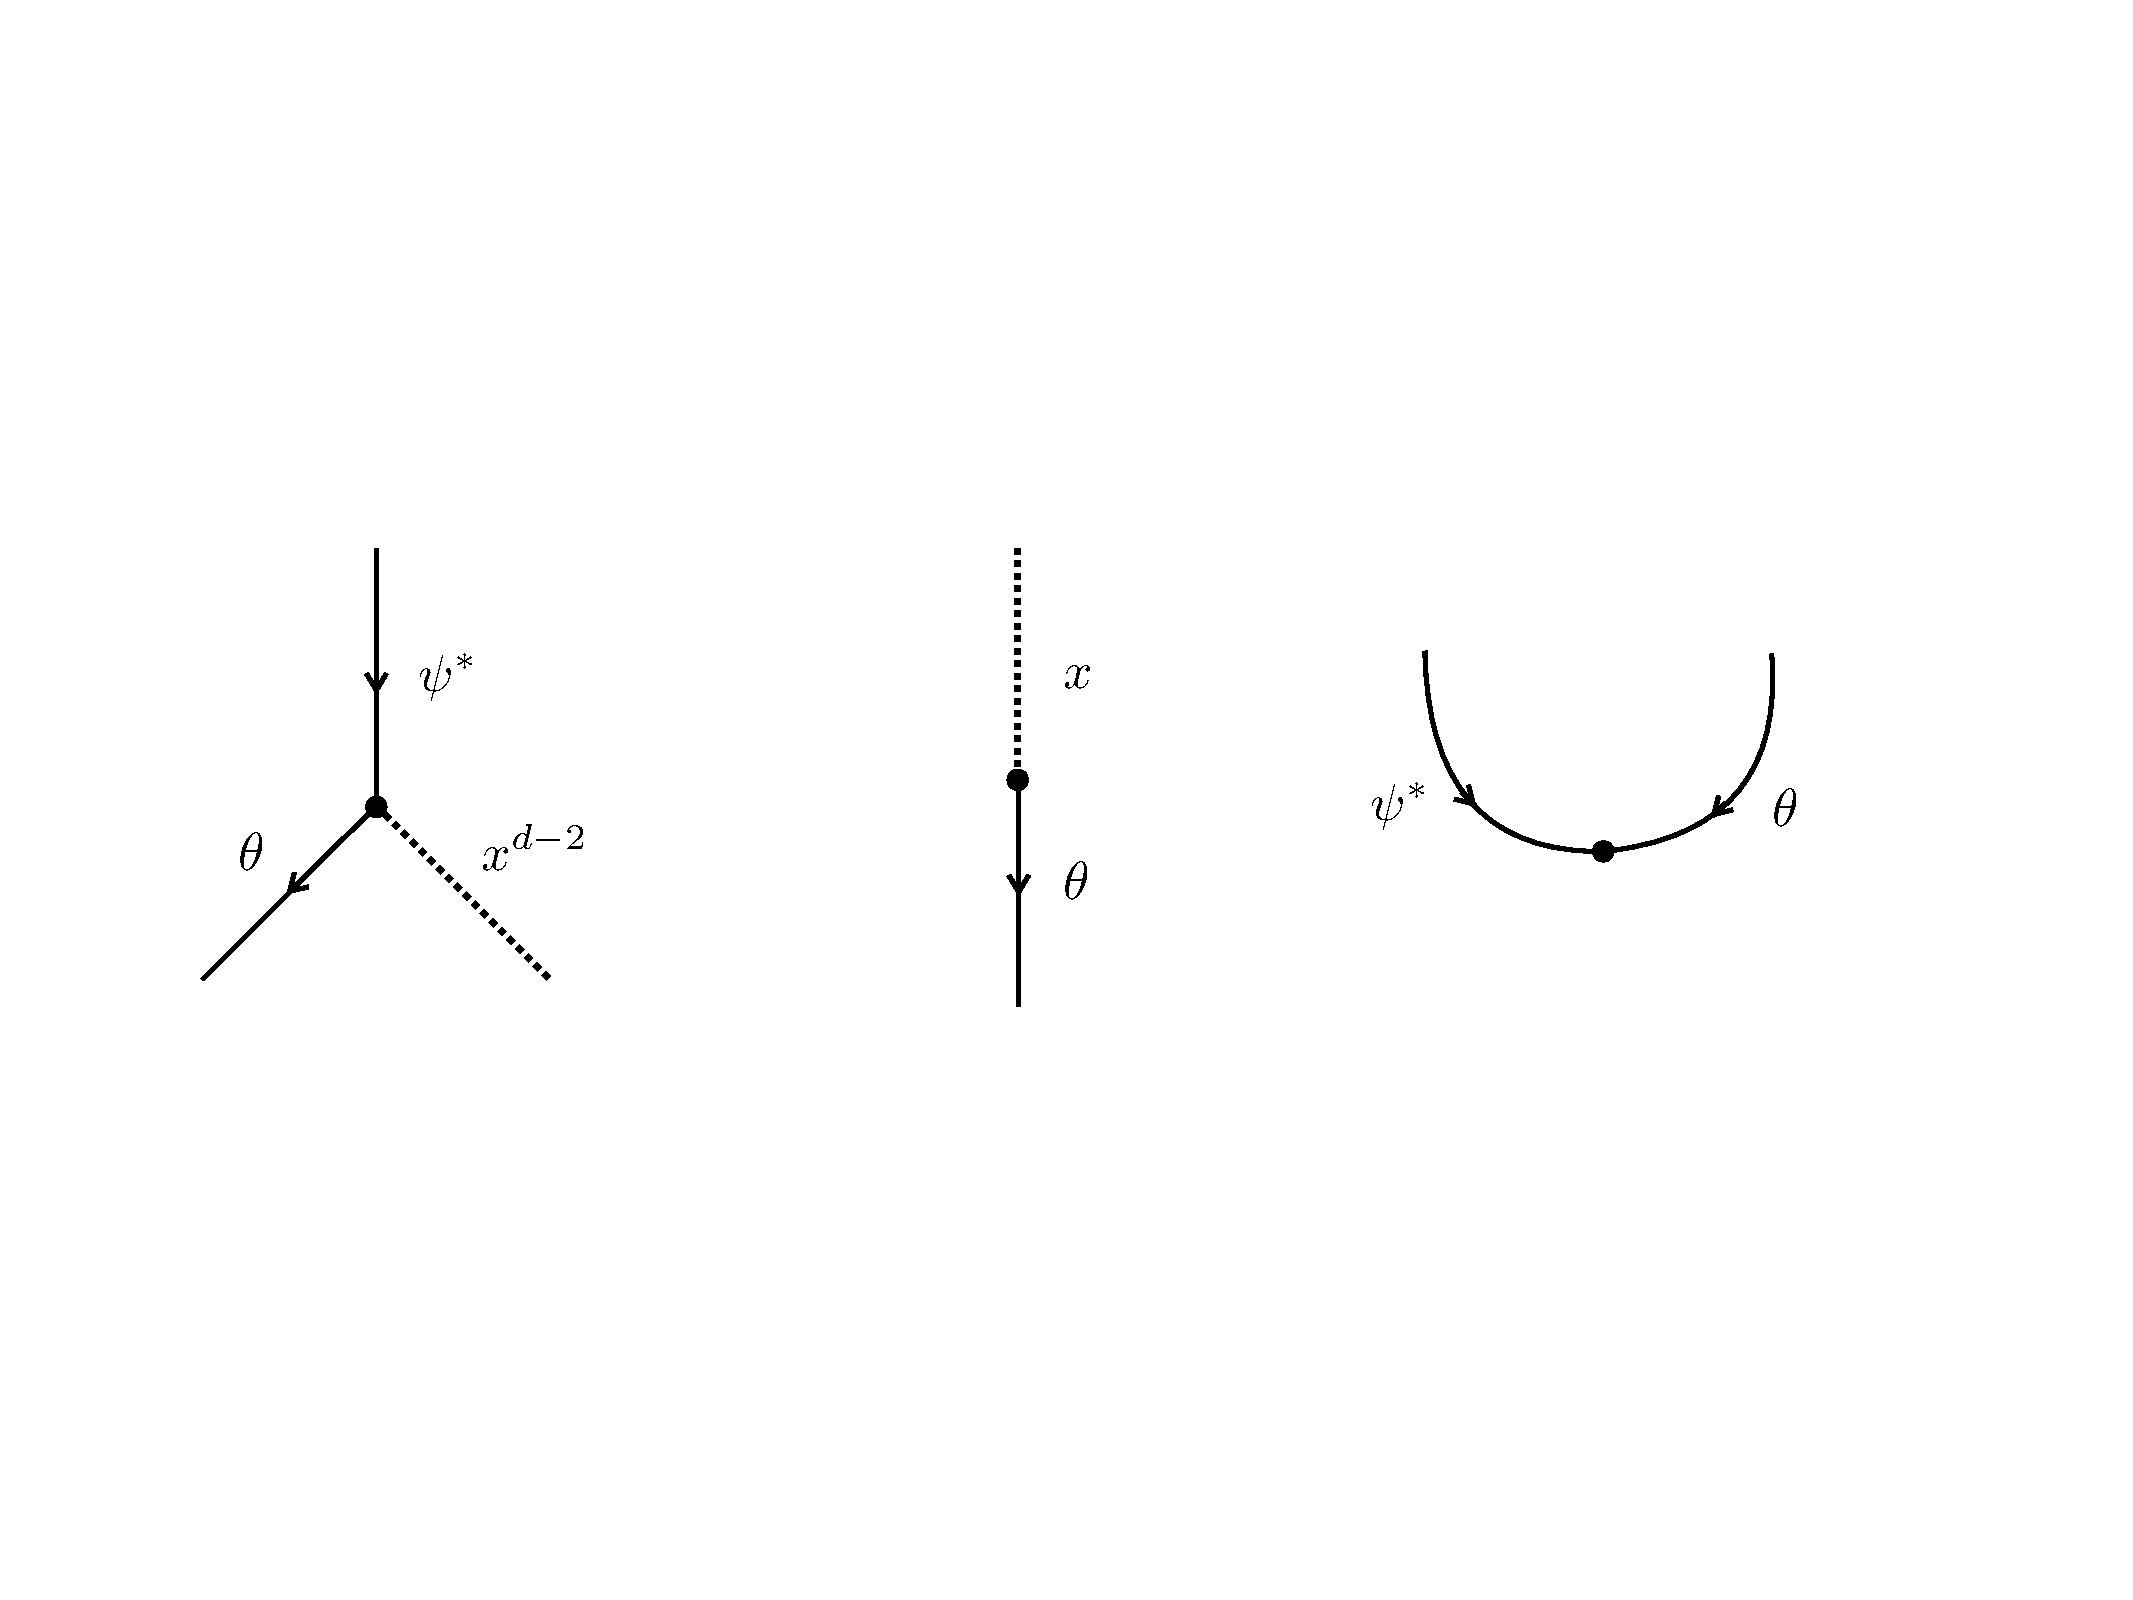
\includegraphics[scale=0.45]{dia9}
\end{center}
Let us compute the $A_\infty$-products $\rho_q$ on $\mathscr{B}$:
\begin{itemize}
\item For $q = 2$ there is only one tree $T \in \cat{T}_2$. We claim that since $T$ has no internal edge the only configuration $C$ with $\cat{O}(T,C) \neq 0$ is the unique $C$ with no A-type or C-type interactions (see Remark \ref{remark:config_count}). To see this, note that an A-type interaction would create a polynomial $x^{d-2}$ which cannot be eliminated by derivatives at internal edges, and therefore annihilates with $p$. Since there can be no A-type interaction to create a $\theta$, the $\theta^*$ in a C-type interaction will end up acting on the identity in the exterior algebra, and giving zero as well. Since this $C$ is the only contributor to the sum, and $\langle D_{T,C} \rangle = p \circ m_2 \circ (\sigma \otimes \sigma)$, we have
\be\label{eq:a_type_product}
\rho_2( \Lambda_2, \Lambda_1 ) = (-1)^{\widetilde{\Lambda_1} \widetilde{\Lambda_2} + \widetilde{\Lambda_1} + 1} \Lambda_1 \cdot \Lambda_2
\ee
where $(-) \cdot (-)$ denotes the usual product in the exterior algebra. This is just the forward suspension of the product in the exterior algebra.

\item For $q > 2$ let $C$ be a configuration with $\cat{O}(T,C) \neq 0$. Then $C$ must have at least one A-type interaction, since otherwise the $\partial_x$ in the B-type interactions are applied to $1 \in R$. Moreover, these A-type interactions can only be inserted at input vertices, since at an internal edge \eqref{eq:int_intedge} would contribute $\theta^2 = 0$.

For the same reason, the $\theta$ coming out of the B-type interaction at an internal edge $e$ must be consumed in a C-type interaction at the vertex $v$ immediately after $e$ on the path to the root: if not, it will annihilate with the $\theta$ emitted at the next internal edge, or, if $v$ is adjacent to the root, it will annihilate with $p$. This means that every edge $e$ must be the right-hand branch at $v$, from which we deduce that $T$ is the tree in which all internal edges lie on the path from the rightmost input to the root:
\begin{center}
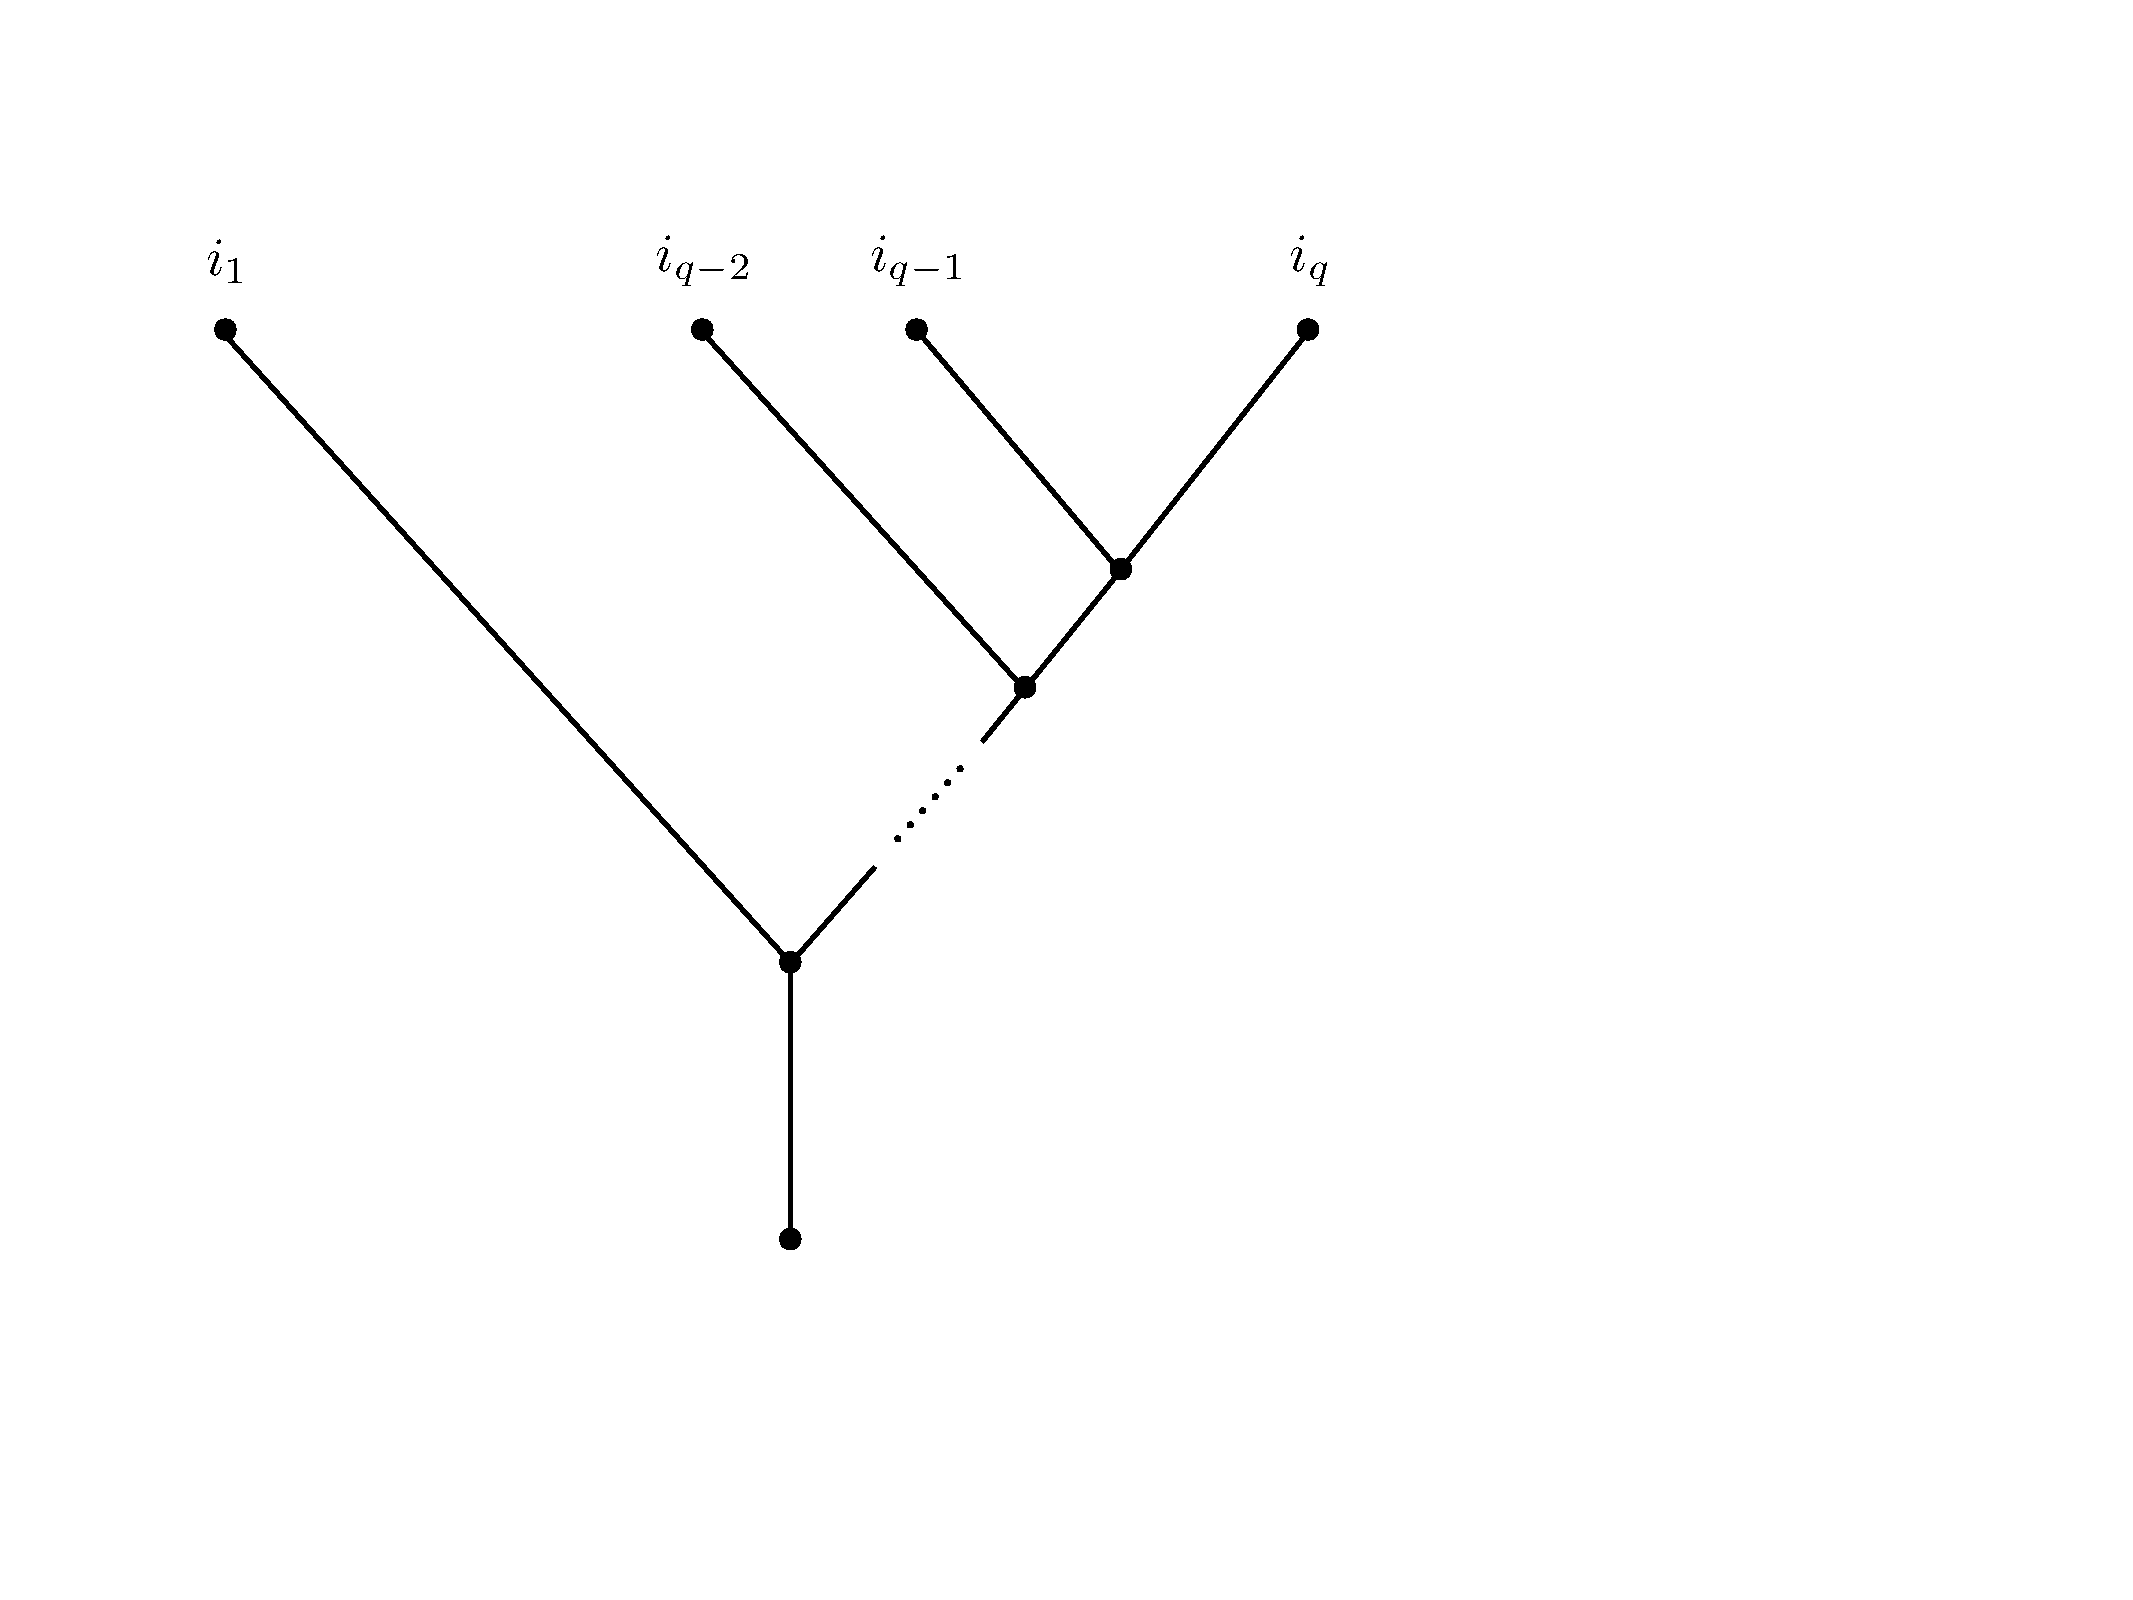
\includegraphics[scale=0.3]{dia10}
\end{center}
This implies that there is \emph{precisely} one A-type interaction in $C$, and it takes place at the vertex marked $i_q$ in the diagram. But since $T$ contains $q - 2$ internal edges, if $\cat{O}(T,C) \neq 0$ then we must have $q = d$. That is, $\rho_q = 0$ unless $q \in \{2,d\}$.

\item Finally, let us describe $\rho_d: \mathscr{B}^{\otimes d} \lto \mathscr{B}$ on the basis of tensors $(\psi^*)^{s_0} \otimes \cdots \otimes (\psi^*)^{s_d}$ where $s_j \in \{0,1\}$ for $1 \le j \le d$. We require a copy of $\psi^*$ at each input $i_1,\ldots,i_{q-2}$ in order to meet the $\theta$ emitted by B-type interactions, a copy of $\psi^*$ at $i_{q-1}$ to meet the $\theta$ from the A-type interaction and a $\psi^*$ at $i_q$ to initiate that A-type interaction. Hence $\rho_d$ is zero on all the basis elements except for
\[
\rho_d( \psi^* \otimes \psi^* \otimes \cdots \otimes \psi^* ) = (-1)^{Q(T, \underline{\Lambda})} \cdot 1\,.
\]
To compute the sign, observe that $e_i(T) = d - 2$ and $\Lambda_i = \psi^*$ is odd so $\widetilde{\Lambda_i}$ is even, whence $Q(T, \underline{\Lambda}) = (d-2) + d + 1 = 1$.
\end{itemize}
In summary: the underlying $\nZ_2$-graded $k$-module of $\mathscr{B}$ is the exterior algebra $\bigwedge( k \psi^* )$ and the $A_\infty$-products $\rho_q$ are zero unless $q \in \{ 2, d \}$. The product $\rho_2$ is the forward suspended version of the usual product on the exterior algebra, while
\[
\rho_d( \psi^* \otimes \psi^* \otimes \cdots \otimes \psi^* ) = -1\,.
\]
\end{example}

\section{The proof}

\subsection{The homotopy retract}

Let $k$ be a characteristic zero field, $R =  k[x_1,\ldots,x_n]$ and let $W \in \mf{m}^3$ be a potential with chosen decomposition $W = \sum_{i=1}^n x_i W^i$. We aim to construct the minimal model of the following DG-algebra
\begin{align*}
\mathscr{A} &= \Big( \End_{R}(k^{\operatorname{stab}}), \; \partial = [d_{k^{\stab}},-] \; \Big)\\
&= \Big( R \otimes_k \End_k\Big( \bigwedge\big( \oplus_i k\psi_i \,\big) \Big),  \partial = \sum_i x_i [\psi_i^*,-] + \sum_i W^i [\psi_i,-] \;\Big)\,.
\end{align*}
Recall the module $\mathscr{H}$ of Definition \ref{defn:handop} which we recall here for the reader's convenience, writing $F = \oplus_i k \psi_i$ for compactness
\[
\mathscr{H} = R \otimes_k \bigwedge\big( \oplus_i k \theta_i \,\big) \otimes_k \End_k\Big( \bigwedge F \Big)\,.
\]
If we extend $\mathscr{A}$ by the exterior algebra on the $\theta$'s we get the DG-algebra
\[
\mathscr{A} \otimes_k \bigwedge\big( \oplus_i k\theta_i \,\big) = \big( \mathscr{H}, \partial \big)\,.
\]
The Koszul complex of the sequence $x_1,\ldots,x_n$ is
\be\label{eq:defnkoszulK}
K = \Big( R \otimes_k \bigwedge\big( \oplus_i k \theta_i \,\big), \; d_K = \sum_i x_i \theta_i^*\; \Big)
\ee
which may be extended by $\End_k\big( \bigwedge F \big)$ to give
\[
K \otimes_k \End_k\big( \bigwedge F \big) = \big( \mathscr{H}, d_K \big)\,.
\]

\begin{definition} The morphism of complexes $\pi: K \lto R/\mf{m}$ is defined by composing the projection of $K$ onto the submodule $R \cdot 1$ of $\theta$-degree zero forms, with the quotient $R \lto R/\mf{m}$. We also write $\pi$ for the following tensor product
\[
\xymatrix@C+2pc{
\big( \mathscr{H}, d_K + \partial \,\big) \ar[r]^-{\pi \otimes 1} & \Big( \End_k\big( \bigwedge F \big), 0 \,\Big)\,.
}
\]
where we use that $R/\mf{m} \otimes_R \End_R(k^{\stab})$ has zero differential by the hypothesis that $W \in \mf{m}^2$. 
\end{definition}

\begin{definition} We write $\sigma$ for the inclusion $\End_k\big( \bigwedge F \big) \lto \mathscr{H}$ defined by
\[
\sigma( \Phi ) = 1 \otimes 1 \otimes \Phi\,.
\]
\end{definition}

\begin{definition}\label{defn:lpsi} Let $L_{\psi_i}$ denote the odd operator on $\End_k\big( \bigwedge F \big)$ defined by
\[
L_{\psi_i}( \alpha ) = \psi_i \circ \alpha = (\psi_i \wedge (-)) \circ \alpha\,,
\]
so that $L_{\psi_i}(\alpha)(x) = \psi_i \wedge \alpha(x)$.
\end{definition}

Throughout $\sum_i$ stands for $\sum_{i=1}^n$.

\begin{theorem}\label{theorem:main_retract} Using the following even homogeneous operators on $\mathscr{H}$,
\be
\delta = \sum_i L_{\psi_i} \theta_i^*\,, \qquad \sigma_\infty = \sum_{m \ge 0} (-1)^m (H \partial)^m \sigma\,,\label{eq:sigmainftyorig}
\ee
and the following odd homogeneous operators
\begin{gather}
\partial = \sum_i x_i [\psi_i^*,-] + \sum_i W^i [\psi_i,-]\,,\\
\nabla = \sum_i \partial_i \theta_i\,, \qquad H = [d_K, \nabla]^{-1} \nabla\,,\label{defn:Horiginal}\\
H_\infty = \sum_{m \ge 0} (-1)^m (H \partial)^m H\,.\label{eq:hinftyorig}
\end{gather}
there is a diagram of $k$-linear homotopy equivalences
\be\label{eq:first_he}
\xymatrix@C+3pc{
\big( \mathscr{H}, \partial \,\big) \ar@<1ex>[r]^-{\exp(-\delta)} & \big( \mathscr{H}, d_K + \partial \,\big) \ar@<1ex>[l]^-{ \exp(\delta) } \ar@<1ex>[r]^-{\pi} & \Big( \End_k\big( \bigwedge F \big), 0 \,\Big)\,.\ar@<1ex>[l]^-{ \sigma_\infty }
}
\ee
More precisely, $\exp(-\delta), \exp(\delta)$ are mutually inverse as $k$-linear maps, $\pi \circ \sigma_\infty = 1$ and
\be
1_{\mathscr{H}} - \big[ d_K + \partial, H_\infty \big] = \sigma_\infty \circ \pi\,.
\ee
\end{theorem}
\begin{proof}
For the duration of the proof let $\mathscr{E} = \End_k\big( \bigwedge F \big)$. It is easy to check that $\exp(\delta),\exp(-\delta)$ intertwines the differentials $\partial$ and $d_K + \partial$ and therefore gives an isomorphism between the first two complexes in \eqref{eq:first_he} \cite[Proposition 4.11]{murfet}. The operator $\psi_j = \psi_j \wedge -$ on $k^{\stab}$ satisfies
\[
[ \psi_j, d_{k^{\stab}} ] = \big[ \psi_j, \sum_i x_i \psi_i^* \big] = x_j \cdot 1\,.
\]
That is, $\psi_j$ is a homotopy for the action of $x_j$ on $k^{\stab}$. It is then easy to check that the odd operator $\alpha \mapsto \psi_j \circ \alpha$ on $\End_R(k^{\stab})$ is also a homotopy for $x_j$.
\end{proof}

It is the homotopy retract \eqref{eq:first_he} that we will ultimately feed into the minimal model theorem, taking as our DG-algebra $(\mathscr{H}, \partial)$ equipped with the projection $\pi \exp(-\delta)$ injection $\exp(\delta) \sigma_\infty$ and the homotopy $\exp(\delta) H_\infty \exp(-\delta)$. In broad outlines, these operators lead to the three types of Feynman diagram interactions as follows:
\begin{itemize}
\item A-type interactions arise from $H_\infty$, more precisely the $H \partial$ factors.
\item B-type interactions arise from the ``odd man out'' $H$ at the right end of $H_\infty$.
\item C-type interactions arise from $\exp(\pm \delta)$.
\end{itemize}
We address each of these in turn before, in Section \ref{??}, finishing the proof.

\subsection{Deriving A-type and B-type interactions}

The A-type and B-type interactions arise from $\sigma_\infty$ and $H_\infty$ from \eqref{eq:sigmainftyorig},\eqref{eq:hinftyorig}. The main task is to understand $(H \partial)^m$. We have for $m > 0$, as an operator on $\mathscr{H}$
\begin{align*}
\big( H \partial )^m &= \prod_{i=1}^m \sum_{j_i = 1}^n H \circ \Big( x_{j_i} [\psi_{j_i}^*,-] + W^{j_i} [\psi_{j_i},-] \Big)\,.
\end{align*}
Prior to Definition \ref{defn:otc} we observed that in calculating $\langle D_{T,C} \rangle$ it suffices to consider operators on the $\nZ_2$-graded $k$-module of $\mathscr{H}$ given by
\be
\mathscr{H}' = R \otimes_k \bigwedge\big( \oplus_{i=1}^n k \theta_i \,\big) \otimes_k \mathscr{B}\,.
\ee
In the next lemma we calculate $(H \partial)^m$ on $\mathscr{H} \cap \Ker(\nabla)$, where $\nabla = \sum_i \partial_i \theta_i$. Before we do this we introduce some notation: in the calculation we use a $\nZ$-grading on $\mathscr{H}'$ defined as follows: $\mathscr{H}'_a$ is the $k$-submodule spanned by tensors of the form
\begin{align*}
f \otimes \omega \otimes \kappa \text{ where } f \in R\,, \omega \in \bigwedge( \oplus_i k \theta_i ), \kappa \in \mathscr{B} \text{ and } |f|_{\nZ} + |\omega|_{\nZ} = a\,.
\end{align*}
Here $|-|_{\nZ}$ denotes the $\nZ$-grading with $|x_i|_{\nZ} = 1$ and $|\theta_i|_{\nZ} = 1$. To be perfectly clear: we have $|\theta_1 \theta_2|_{\nZ} = 2$, as compared to $| \theta_1 \theta_2 | = 0$ in the $\nZ_2$-grading used elsewhere in the text.

\begin{lemma}\label{lemma:commutator_numberop} If $f \in R$ and $\omega \in \bigwedge( \oplus_{i=1}^n k \theta_i )$ are homogeneous then
\be
[d_K, \nabla]( f \otimes \omega ) = ( |f|_{\nZ} + |\omega|_{\nZ} ) f \otimes \omega\,.
\ee
\end{lemma}

\begin{proposition}\label{prop:hpartialmrestrict} Restricted to $\mathscr{H}'_a \cap \Ker(\nabla)$, $(H \partial)^m$ is equal to
\be\label{eq:hpartialmrestrict}
\sum_{\substack{1 \le j_1 < \cdots < j_m \le n \\ 1 \le z_1 < \cdots < z_m \le n \\ \gamma_1,\ldots,\gamma_m \in \mathbb{N}^n \setminus \{0\}}} \sum_{\nu \in \mathfrak{S}_m} \frac{\zeta_{a}( |\gamma_1|,\ldots,|\gamma_m| )}{|\gamma_1| \cdots |\gamma_m|} \prod_{i=1}^m W^{j_i}(\gamma_i) \partial_{z_{\nu(i)}}(x^{\gamma_i}) \theta_{z_{\nu(i)}} [ \psi_{j_i}, - ]\,.
\ee
\end{proposition}
\begin{proof}
On this submodule of $\mathscr{H}$ the operators $[\psi_i^*,-]$ act as zero, and so $(H \partial)^m$ takes a simpler form. If $\underline{j}$ ranges over sequences of length $m$ in $\{1,\ldots,n\}^m$ and $\underline{\gamma}$ over sequences of length $m$ in $\mathbb{N}^n$ then
\begin{align*}
\big( H \partial )^m \arrowvert_{\mathscr{H}'} &= \sum_{\underline{j}} \prod_{i=1}^m H \circ \Big( W^{j_i} [ \psi_{j_i}, - ] \Big)\\
&= \sum_{\underline{j}} \prod_{i=1}^m H \circ \Big( \sum_{\gamma_i} W^{j_i}(\gamma_i) x^{\gamma_i} [ \psi_{j_i}, - ] \Big)\\
&= \sum_{\underline{j}, \underline{\gamma}} \prod_{i=1}^m H \circ \Big( W^{j_i}(\gamma_i) x^{\gamma_i} [ \psi_{j_i}, - ] \Big)\\
&= \sum_{\underline{j}, \underline{\gamma}} \prod_{i=1}^m [d_K, \nabla]^{-1} \nabla \circ \Big( W^{j_i}(\gamma_i) x^{\gamma_i} [ \psi_{j_i}, - ] \Big)\,.
\end{align*}
Note that $W^i$ contains no constant term, since by hypothesis $W \in \mf{m}^2$, so in fact we may assume that all $\gamma_i$ are nonzero. Our convention is that products of operators expand from left to right as $i$ increases. Lemma \ref{lemma:commutator_numberop}

Now we consider the scalar factors produced by the $[d_K, \nabla]^{-1}$ when we apply $(H \partial)^m$ to a tensor $f \otimes \omega \otimes \Psi$. Observe how the sum of the polynomial and $\theta$-degree changes with each application of $H \partial$. Multiplying with $x^{\gamma_i}$ increases the polynomial degree by $|\gamma_i|$, while applying $\nabla$ decreases the polynomial degree and increases the $\theta$-degree by one, so overall the $i$th copy of $H \partial$ (reading from left to right) increases the sum of the two degrees from
\[
|f|_{\nZ} + |\omega|_{\nZ} + \sum_{t > i} |\gamma_t| \qquad \text{ to } \qquad |f|_{\nZ} + |\omega|_{\nZ} + \sum_{t \ge i} |\gamma_t|\,.
\]
If we write $a = |f| + |\omega|$ then the scalar factor contributed by the copies of $[d_K, \nabla]^{-1}$ in $(H \partial)^m$ applied to $f \otimes \omega \otimes \Psi$ is therefore
\[
\frac{1}{(a + |\gamma_m|)(a + |\gamma_m| + |\gamma_{m-1}|) \cdots (a + |\gamma_m| + \cdots + |\gamma_1|)}\,.
\]
This leads us to the un-symmetrised version of $\zeta$ from Definition \ref{defn:zeta}: given a sequence $a_1,\ldots,a_m \ge 1$ of integers and $a \ge 0$ we define
\be\label{defn:zeta_unsym}
\zeta'_a(a_1,\ldots,a_m) = \frac{1}{(a + a_m)(a + a_{m-1} + a_m) \cdots (a + a_1 + \cdots + a_m)}\,.
\ee
Let $\mathscr{H}'_a \subseteq \mathscr{H}'$ denote the submodule of elements of degree $a$, when we take the $\nZ$-grading induced by the usual $\nZ$-grading on $R$ and the exterior algebra in the $\theta$'s (so, the grading does not count $\psi$'s). Then we have computed that
\be
(H \partial)^m|_{\mathscr{H}'_a} = \sum_{\underline{j}, \underline{\gamma}} \zeta'_{a}( |\gamma_1|, \ldots, |\gamma_m| ) \prod_{i=1}^m \nabla \circ \big( W^{j_i}(\gamma_i)x^{\gamma_i} [ \psi_{j_i}, - ] \big) \,.
\ee
For a $k$-linear operator $T$ and an element $x \in \Ker(\nabla)$ since $\nabla^2 = 0$ we have
\[
\nabla T \cdots \nabla T (x) = [\nabla, T] \cdots [\nabla, T](x)\,.
\]
Using $[ \nabla, f ] = \sum_q \partial_q(f) \theta_q$ we therefore have
\begin{align*}
\big( H \partial )^m|_{\mathscr{H}'_a \cap \Ker(\nabla)} &= \sum_{\underline{j}, \underline{\gamma}} \zeta'_{a}( |\gamma_1|, \ldots, |\gamma_m| ) \prod_{i=1}^m \Big[ \nabla, W^{j_i}(\gamma_i)x^{\gamma_i} [ \psi_{j_i}, - ] \Big]\\
&= \sum_{\underline{j}, \underline{\gamma},\underline{z}} \zeta'_{a}( |\gamma_1|, \ldots, |\gamma_m| ) \prod_{i=1}^m W^{j_i}(\gamma_i) \partial_{z_i}(x^{\gamma_i}) \theta_{z_i} [ \psi_{j_i}, - ]
\end{align*}
where $\underline{j},\underline{z}$ both range over $\{1, \ldots, n\}^m$. Since $[ \psi_j, - ]^2 = 0$ the only nonzero contributions are from sequences $\underline{j} = (j_1,\ldots,j_m)$ without repeats and similarly for $\underline{z}$. Thus
\begin{align*}
&= \sum_{\substack{j_1 < \cdots < j_m \\ z_1 < \cdots < z_m}} \sum_{\rho,\nu \in \mathfrak{S}_m} \sum_{\underline{\gamma}} \zeta'_{a}( |\gamma_1|, \ldots, |\gamma_m| ) \prod_{i=1}^m W^{j_{\rho(i)}}(\gamma_i) \partial_{z_{\nu(i)}}(x^{\gamma_i}) \theta_{z_{\nu(i)}} [ \psi_{j_{\rho(i)}}, - ]\\
&= \sum_{\substack{j_1 < \cdots < j_m \\ z_1 < \cdots < z_m}} \sum_{\rho,\nu \in \mathfrak{S}_m} \sum_{\underline{\gamma}} \zeta'_{a}( |\gamma_1|, \ldots, |\gamma_m| ) \prod_{i=1}^m W^{j_i}(\gamma_{\rho^{-1}(i)}) \partial_{z_{\nu\rho^{-1}(i)}}(x^{\gamma_{\rho^{-1}(i)}}) \theta_{z_{\nu\rho^{-1}(i)}} [ \psi_{j_i}, - ]\\
&= \sum_{\substack{j_1 < \cdots < j_m \\ z_1 < \cdots < z_m}} \sum_{\rho,\nu \in \mathfrak{S}_m} \sum_{\underline{\gamma}} \zeta'_{a}( |\gamma_{\rho(1)}|, \ldots, |\gamma_{\rho(m)}| ) \prod_{i=1}^m W^{j_i}(\gamma_i) \partial_{z_{\nu(i)}}(x^{\gamma_i}) \theta_{z_{\nu(i)}} [ \psi_{j_i}, - ]\\
&= \sum_{\substack{j_1 < \cdots < j_m \\ z_1 < \cdots < z_m}} \sum_{\nu \in \mathfrak{S}_m} \sum_{\underline{\gamma}} \frac{\zeta_{a}( |\gamma_1|,\ldots,|\gamma_m| )}{|\gamma_1| \cdots |\gamma_m|} \prod_{i=1}^m W^{j_i}(\gamma_i) \partial_{z_{\nu(i)}}(x^{\gamma_i}) \theta_{z_{\nu(i)}} [ \psi_{j_i}, - ]
\end{align*}
%That is, if we write
%\[
%Y = \{ ( z, \gamma ) \l 1 \le z \le n\,, \gamma \in \mathbb{N}^m\,, \gamma_z \ge 1 \}
%\]
%then
as claimed.
\end{proof}

\begin{remark} Since $\nabla \sigma = 0$ and $\nabla^2 = 0$ the proposition applies to calculate $\sigma_\infty, H_\infty$. In the former case we simply append $\sigma$ and use \eqref{eq:sampzero} to see that $(H \partial)^m \sigma$ is given under the same summation over $\underline{j},\underline{z},\underline{\gamma}, \nu$ as in \eqref{eq:hpartialmrestrict} by
\be
\sum_{\underline{j},\underline{z},\underline{\gamma},\nu} \frac{1}{|\gamma_1| \cdots |\gamma_m|} \Big\{ \prod_{i=1}^m W^{j_i}(\gamma_i) \partial_{z_{\nu(i)}}(x^{\gamma_i}) \theta_{z_{\nu(i)}} [ \psi_{j_i}, - ] \Big\} \circ \sigma\,.
\ee
In the case of $H_\infty$ we observe that $H = [d_K, \nabla]^{-1} \nabla$ sends $\mathscr{H}'_a$ into $\mathscr{H}'_a \cap \Ker(\nabla)$, and we have that $(H \partial)^m H$ on $\mathscr{H}'_a$ is given by
\be
\sum_{\underline{j},\underline{z},\underline{\gamma},\nu} \sum_{t = 1}^n \frac{1}{a} \frac{\zeta_{a}( |\gamma_1|,\ldots,|\gamma_m| )}{|\gamma_1| \cdots |\gamma_m|} \Big\{ \prod_{i=1}^m W^{j_i}(\gamma_i) \partial_{z_{\nu(i)}}(x^{\gamma_i}) \theta_{z_{\nu(i)}} [ \psi_{j_i}, - ] \Big\} \circ \partial_t \theta_t\,.
\ee
\end{remark}

\begin{remark}\label{remark:virt_part_2} Continuing from Remark \ref{remark:virtual_part} we note that in contrast to the way we usually think about the minimal model construction in the setting of topological string theory \cite{??} the elements $\Psi$ of $\mathscr{B}$ are not immediately identified with cohomology classes of $\mathscr{B}$. 

Of course $\sigma_\infty(\Psi)$ is a cycle for $\partial$, but this is already given by a complicated sum which contributes multiple Feynman diagrams in the calculus of Definition \ref{??}. That is to say, we have found it useful for purposes of calculation to have the incoming states in our Feynman diagrams to be elements of $\mathscr{H}$ that are \emph{not} cycles. Note that as we vary the potential $W$ the elements of $\mathscr{H}$ that are cycles will change - this makes it awkward to take as a starting point the cohomology of $\mathscr{H}$. In our approach the subspace $\mathscr{B}$ remains fixed, and even in the case of quadratic terms it is only the projection to $\mathscr{B}$ that changes.
\end{remark}

\subsection{Deriving C-type interactions}
% see ainfmf4

Let us briefly recall some of the notation from earlier: we write $F = \oplus_i k \psi_i$ and use the operators $L_{\psi_i}$ of Definition \ref{defn:lpsi} and $\delta$ of \eqref{eq:sigmainftyorig}. We set $\delta_i = L_{\psi_i} \theta_i^*$ so that $\delta = \sum_i \delta_i$. To be explicit, given $\omega_i \in \bigwedge( \oplus_i k \theta_i )$ and $\kappa_i \in \End_k(\bigwedge F)$
\[
\delta_i( \omega \otimes \kappa ) = L_{\psi_i}\big( \theta_i^*( \omega ) \otimes \kappa ) = (-1)^{|\omega| + 1} \theta_i^*(\omega) \otimes \psi_i \circ \kappa\,.
\]

\begin{lemma}\label{lemma:stratos} For $1 \le i \le n$ there is a commutative diagram
\be
\xymatrix@C+3pc@R+1pc{
\mathscr{H} \otimes_k \mathscr{H} \ar[d]_-{\delta_i \otimes 1 + 1 \otimes \delta_i + [\psi_i,-] \otimes \theta_i^*} \ar[r]^-{m_2} & \mathscr{H} \ar[d]^-{\delta_i}\\
\mathscr{H} \otimes_k \mathscr{H} \ar[r]_-{m_2} & \mathscr{H}
}
\ee
\end{lemma}
\begin{proof}
By direction calculation: given $\omega_j \in \bigwedge( \oplus_i k \theta_i )$ and $\kappa_j \in \bigwedge( \oplus_i k \psi_i )$
\begin{align*}
&m_2\big( \delta_i \otimes 1 + 1 \otimes \delta_i \big)( \omega_1 \otimes \kappa_1 \otimes \omega_2 \otimes \kappa_2 )\\
&= m_2\big( \delta_i( \omega_1 \otimes \kappa_1 ) \otimes \omega_2 \otimes \kappa_2 \big)\\
&+ m_2\big( \omega_1 \otimes \kappa_1 \otimes \delta_i( \omega_2 \otimes \kappa_2 ) \big)\\
&= (-1)^{|\omega_1| + 1}m_2\big( \theta_i^*(\omega_1) \otimes \psi_i \circ \kappa_1 \otimes \omega_2 \otimes \kappa_2 )\\
&+ (-1)^{|\omega_2| + 1}m_2\big( \omega_1 \otimes \kappa_1 \otimes \theta_i^*(\omega_2) \otimes \psi_i \circ \kappa_2 \big)\\
&= (-1)^{|\omega_1|+1+(|\kappa_1|+1)|\omega_2|} \theta_i^*(\omega_1) \omega_2 \otimes \psi_i \circ \kappa_1 \circ \kappa_2\\
&+ (-1)^{|\omega_2|+1+(|\omega_2|+1)|\kappa_1|} \omega_1 \theta_i^*(\omega_2) \otimes \kappa_1 \circ \psi_i \circ \kappa_2
\end{align*}
Similarly one computes
\begin{align*}
&m_2 \big( [\psi_i,-] \otimes \theta_i^* \big)( \omega_1 \otimes \kappa_1 \otimes \omega_2 \otimes \kappa_2 \big)\\
&= (-1)^{|\kappa_1|} m_2 \big( \omega_1 \otimes [\psi_i, \kappa_1] \otimes \theta_i^*(\omega_2) \otimes \kappa_2 \big)\\
&= (-1)^{|\kappa_1|+(|\kappa_1|+1)(|\omega_2|+1)} \omega_1 \theta_i^*(\omega_2) \otimes [\psi_i, \kappa_1] \circ \kappa_2\,.
\end{align*}
Adding these together yields that $\delta_i \otimes 1 + 1 \otimes \delta_i + [\psi_i,-] \otimes \theta_i^*$ on $\omega_1 \otimes \kappa_1 \otimes \omega_2 \otimes \kappa_2$ is
\begin{align*}
&= (-1)^{|\omega_1|+1+(|\kappa_1|+1)|\omega_2|} \theta_i^*(\omega_1) \omega_2 \otimes \psi_i \circ \kappa_1 \circ \kappa_2\\
&+ (-1)^{|\kappa_1|+(|\kappa_1|+1)(|\omega_2|+1)} \omega_1 \theta_i^*(\omega_2) \otimes \psi_i \circ \kappa_1 \circ \kappa_2\\
&= (-1)^{|\omega_1|+|\omega_2|+|\kappa_1||\omega_2|+1} \theta_i^*( \omega_1 \omega_2 ) \otimes \psi_i \circ \kappa_1 \circ \kappa_2\\
&= (-1)^{|\kappa_1||\omega_2|}\delta_i\big( \omega_1 \omega_2 \otimes \kappa_1 \circ \kappa_2 \big)\\
&= \delta_i \circ m_2\big( \omega_1 \otimes \kappa_1 \otimes \omega_2 \otimes \kappa_2 \big)
\end{align*}
as claimed.
\end{proof}

\begin{definition} We define $\Xi_i = [ \psi_i, - ] \otimes \theta_i^* : \mathscr{H}^{\otimes 2} \lto \mathscr{H}^{\otimes 2}$ and $\Xi = \sum_i \Xi_i$. 
\end{definition}

\begin{lemma}\label{lemma:somecommt} As operators on $\mathscr{H} \otimes_k \mathscr{H}$, for all $1 \le i,j \le n$
\begin{align}
\big[ \delta_i \otimes 1, 1 \otimes \delta_j \big] &= 0\\
\big[ \delta_i \otimes 1, \Xi_j \big] &= 0\\
\big[ 1 \otimes \delta_i, \Xi_j \big] &= 0\,.
\end{align}
\end{lemma}

\begin{proposition}\label{prop:adamant} There is a commutative diagram
\be
\xymatrix@C+3pc@R+2pc{
\mathscr{H} \otimes \mathscr{H} \ar[d]_-{\exp(-\delta) \otimes \exp(-\delta)} \ar[r]^-{m_2} & \mathscr{H} \ar[dd]^-{\exp(-\delta)}\\
\mathscr{H} \otimes \mathscr{H} \ar[d]_-{\exp(-\Xi)}\\
\mathscr{H} \otimes \mathscr{H} \ar[r]_-{m_2} & \mathscr{H}
}
\ee
\end{proposition}
\begin{proof}
By Lemma \ref{lemma:somecommt} we have
\[
\exp\big(-\big[ \delta_i \otimes 1 + 1 \otimes \delta_i + \Xi_i \big]\big) = \exp(-\Xi_i) \circ \big\{ \exp(-\delta_i) \otimes \exp(-\delta_i) \big\}
\]
and therefore
\[
\exp\big(-\big[ \delta \otimes 1 + 1 \otimes \delta + \Xi \big]\big) = \exp(-\Xi) \circ \big\{ \exp(-\delta) \otimes \exp(-\delta) \big\}\,.
\]
By Lemma \ref{lemma:stratos} then
\begin{align*}
\exp(-\delta) m_2 &= \sum_{m \ge 0} (-1)^m \frac{1}{m!} \delta^m m_2\\
&= \sum_{m \ge 0} (-1)^m \frac{1}{m!} m_2 \big\{ \delta \otimes 1 + 1 \otimes \delta + \Xi \big\}^m\\
&= m_2 \exp\big(-\big[ \delta \otimes 1 + 1 \otimes \delta + \Xi \big] \big)\\
&= m_2 \exp(-\Xi) \circ \big\{ \exp(-\delta) \otimes \exp(-\delta) \big\}\,,
\end{align*}
which completes the proof.
%Immediately from \eqref{eq:graded_jacobi} and \eqref{eq:wedge_contract_comm} we have
%\begin{align*}
%\big[ [ \varepsilon_i^*, -], \varepsilon_j \big] &= \big[ [ \varepsilon_i, - ], \varepsilon_j^* \big] = \delta_{ij} \cdot 1\,.\\
%\big[[ \varepsilon_i^*, -], \varepsilon_j^* \big] &= \big[[\varepsilon_i, -], \varepsilon_j\big] = 0\,.
%\end{align*}
\end{proof}

Observe finally that
% see ainfmf9 p.14
\be
\exp(-\Xi) = \sum_{m \ge 0} (-1)^m \sum_{1 \le j_1 < \cdots < j_m \le n} \prod_{i=1}^m \;[\psi_{j_i},-] \otimes \theta_{j_i}^*\,.
\ee

\subsection{Atiyah classes and idempotents}
% ainfmf12

The endomorphism algebra $C = \End_k(S)$ is a Clifford algebra generated by the contraction $\theta_i^*$ and wedge product $\theta_i$ operators. It is observed in \cite{murfet} that \eqref{eq:he_start} is an isomorphism of Clifford representations (in the homotopy category) when the complex $\md{E}$ is equipped with the action induced by Atiyah classes:

\begin{definition}
The Atiyah classes of $\md{A}_W$ are the $R$-linear odd operators
\[
\At_i = [\partial, \partial_{i}]: \End_R(k^{\stab}) \lto \End_R(k^{\stab})\,,
\]
\end{definition}

\begin{lemma} We have
\[
\At_i = -[\psi_i^*, -] - \sum_{q=1}^n \partial_{i}(W^q) [ \psi_q, - ]\,.
\]
\end{lemma}
\begin{proof}
By direct calculation:
\begin{align*}
\At_i &= \big[ [d_{k^{\stab}},-], \partial_{i} \big]\\
&= \sum_q \big[x_q [\psi_q^*,-], \partial_{i}\big] + \sum_q \big[W^q [\psi_q,-], \partial_{i}\big]\\
&= -\sum_q \partial_{i}(x_q) [\psi_q^*,-] - \sum_q \partial_{i}(W^q) [\psi_q,-]\\
&= -[\psi_i^*,-] - \sum_q \partial_{i}(W^q) [\psi_q, -]\,.
\end{align*}
\end{proof}

\begin{lemma} The induced Clifford algebra structure on $\mathscr{E}$ is given by
\[
\gamma_i^\dagger = \At_i = -[\psi_i^*, -]\,, \qquad \gamma_i = -\psi_i\,.
\]
\end{lemma}

\begin{lemma} The idempotent $e = \gamma_1^\dagger \cdots \gamma_n^\dagger \gamma_n \cdots \gamma_1$ is the projection onto $\mathscr{B} \subseteq \mathscr{E}$.
\end{lemma}


\subsection{Putting it all together}

In this section we put together all the earlier elements, and prove the description of the minimal model of $\mathscr{A}$ given in Section \ref{??}. In this section we write
\[
\mathscr{E} = \End_k\Big( \bigwedge( \oplus_i k \psi_i ) \Big)\,.
\]
The starting point is Theorem \ref{theorem:main_retract}, which gives us a strong deformation retract
\be\label{eq:ho_retract_for_mm}
\xymatrix@C+5pc{
\big( \mathscr{H}, \partial \,\big) \ar@<1ex>[r]^-{\pi\exp(-\delta)} & \big( \mathscr{E}, 0 \big) \ar@<1ex>[l]^-{ \exp(\delta)\sigma_\infty }
}
\ee
with $\pi \exp(-\delta) \circ \exp(\delta) \sigma_\infty = 1$ and
\[
\exp(\delta)\sigma_\infty \pi\exp(-\delta) = 1 - \big[ \partial, \exp(\delta) H_\infty \exp(-\delta) \big]\,.
\]

\begin{definition} Let $\xi_q$ denote the product $\xi_q: \mathscr{E}[1]^{\otimes q} \lto \mathscr{E}[1]$ induced by the homotopy retract \eqref{eq:ho_retract_for_mm} and the minimal model construction, defining an $A_\infty$-structure on $\mathscr{E}$. That is,
\[
\xi_q = \sum_{T \in \cat{T}_q} (-1)^{e_i(T)} \langle D_T \rangle
\]
where $D_T$ is the decoration given by the assignment of modules
\begin{itemize}
\item $\mathscr{E}$ to each leaf including the root, and
\item $\mathscr{H}$ to each edge.
\end{itemize}
To each vertex $v$ of $A(T)$ we associate an operator $\phi_v$ as follows:
\begin{itemize}
\item if $v$ is an input, then $\phi_v = \exp(\delta)\sigma_\infty$.
\item if $v$ comes from an internal edge of $T$, then $\phi_v = \exp(\delta)H_\infty\exp(-\delta)$.
\item if $v$ comes from an internal vertex of $T$, then $\phi_v = r_2$ where $r_2$ is the forward suspension of the product $m_2$ in $\mathscr{H}$, that is,
\be\label{eq:r2vsm2}
r_2( \alpha \otimes \beta ) = (-1)^{\widetilde{\alpha}\widetilde{\beta} + \widetilde{\beta} + 1} m_2( \beta \otimes \alpha )\,.
\ee
\item if $v$ is the root, then $\phi_v = \pi \exp(-\delta)$.
\end{itemize}
\end{definition}

\begin{proposition} For $q \ge 2$
\be
\xi_q( \Lambda_q, \ldots, \Lambda_1 ) = \sum_{T \in \cat{T}_q} (-1)^{Q(T, \Lambda_1, \ldots, \Lambda_q)} \langle D'_T \rangle( \Lambda_1,\ldots,\Lambda_q)
\ee
where $Q(T, \Lambda_1, \ldots, \Lambda_q)$ is as in \eqref{eq:defnQsign}, and $D'_T$ is the decoration of $A(T)$ assigning $\mathscr{E}$ to each leaf and $\mathscr{H}$ to each edge, and to each vertex $v$ the operator $\phi_v$ defined as follows:
\begin{itemize}
\item if $v$ is an input, then $\phi_v = \sigma_\infty$.
\item if $v$ comes from an internal edge of $T$, then $\phi_v = H_\infty$.
\item if $v$ comes from an internal vertex of $T$, then
\[
\phi_v = m_2 \circ \exp(- \Xi)\,.
\]
\item if $v$ is the root, then $\phi_v = \pi$.
\end{itemize}
\end{proposition}
\begin{proof}
The substitution of $m_2$ for $r_2$ incurs some sign factors and reverses the order of the inputs, and we will return to this sign at the end. We prove the proposition by taking the ``extra'' $\exp(-\delta)$ factor at the root and moving it upwards in the tree: at the vertex $v$ adjacent to the root, we use Proposition \ref{prop:adamant} to see that
\[
\exp(-\delta) \circ m_2 = m_2 \circ \exp(-\Xi) \circ (\exp(-\delta) \otimes \exp(-\delta))\,,
\]
which replaces the $m_2$ at the vertex by $m_2 \circ \exp(-\Xi)$ and propagates the $\exp(-\delta)$ factors to the edges adjacent and above $v$.  internal this extra factor has the effect of
\[
\exp(-\delta) \circ \exp(\delta) H_\infty \exp(-\delta) = H_\infty \exp(-\delta)
\] 
leaving behind a $H_\infty$ and moving upwards, while in the case of an external edge
\[
\exp(-\delta) \circ \exp(\delta) \sigma_\infty = \sigma_\infty
\]
we are left with a bare $\sigma_\infty$.

Now to return to the signs, which come from \eqref{eq:r2vsm2} applied at every internal vertex of $T$, when evaluating $\xi_q( \Lambda_q, \ldots, \Lambda_1 )$. The labels $\exp(\delta) H_\infty \exp(-\delta)$ and $r_2$ on internal edges and vertices have degree $+1$ with respect to the tilde grading, which means that when a $\Lambda_i$ reaches an internal vertex of $T$ it is still carrying the same tilde grading $\widetilde{\Lambda_i}$.

It follows that the $\widetilde{\alpha}\widetilde{\beta}$ part of $\eqref{eq:r2vsm2}$ contributes overall $\sum_{i < j} \widetilde{\Lambda_i} \widetilde{\Lambda_j}$ while the $\widetilde{\beta}$ part contributes $\sum_i \widetilde{\Lambda_i} C_i$, and the $1$ contributes $q - 1$, the number of internal vertices.
\end{proof}

\newpage

\bibliographystyle{amsalpha}
\providecommand{\bysame}{\leavevmode\hbox to3em{\hrulefill}\thinspace}
\providecommand{\href}[2]{#2}
\begin{thebibliography}{BHLS03}
  
  \bibitem[Dyc11]{d0904.4713}
T.~Dyckerhoff, \textsl{Compact generators in categories of matrix factorizations},
  Duke Math. J. \textbf{159} (2011), 223--274,
  \href{http://arxiv.org/abs/0904.4713}{[arXiv:0904.4713]}.
  
\bibitem{lazaroiu}
C.~I.~Lazaroiu, \textsl{Generating the superpotential on a D-brane category: I}, [arXiv:hep-th/0610120].

\bibitem{lazaroiu2}
C.~I.~Lazaroiu, \textsl{String field theory and brane superpotentials}.
  
\bibitem{murfet}
D.~Murfet, \textsl{Computing with cut systems}, \href{http://arxiv.org/abs/1402.4541}{[arXiv:1402.4541]}.

\bibitem{lgdual}
N.~Carqueville and D.~Murfet, \textsl{Adjunctions and defects in Landau-Ginzburg models}, Adv. Math. \textbf{289} (2016), 480--566.

\bibitem{dm1102.2957}
T.~Dyckerhoff and D.~Murfet, \textsl{Pushing forward matrix factorisations}, Duke Math. J. \textbf{162} (2013), 1249--1311.

\bibitem{weinberg}
Weinberg, \textsl{The Quantum Theory of Fields Volume 1}.

\bibitem{ps}
Peskin \& Shroeder, \textsl{An introduction to QFT}.

\bibitem{sullivan}
D.~Sullivan, \textsl{Open and closed string field theory interpreted in classical algebraic topology} London Math. Soc. Lecture Note Series 308 (2004).

\bibitem{qftstring}
P.~Deligne et al, \textsl{Quantum fields and strings}

\bibitem{EGA4}
A.~Grothendieck, \textsl{\'{E}l\'ements de g\'eom\'etrie alg\'ebrique. {IV}. \'{E}tude
  locale des sch\'emas et des morphismes de sch\'emas}, Inst.~Hautes \'Etudes
  Sci.~Publ.~Math.~(1964), no.~20.

\bibitem{stacks_project}
The Stacks Project, \href{http://stacks.math.columbia.edu/}{http://stacks.math.columbia.edu}.

\bibitem{matsumura}
Matsumura, \emph{book}.

\bibitem{eisenbudharris}
Eisenbud, David, and Joe Harris. The geometry of schemes. Vol. 197. Springer Science \& Business Media, 2006.

\end{thebibliography}

\end{document}